



\documentclass[a4paper,twoside,openright]{report}

\usepackage[utf8]{inputenc} 
\usepackage[english]{babel}
\usepackage{amssymb,amsfonts}
\usepackage[dvips]{graphicx}
\usepackage{fancyhdr}
\usepackage[linesnumbered,ruled]{VignetteDir/algorithm2e}
\usepackage{epsfig}
\usepackage{rotating,booktabs}
\usepackage{graphicx,subfigure}
\usepackage{amsmath}
\usepackage{path}
\usepackage[colorlinks=true,anchorcolor=blue,backref=page,ps2pdf]{hyperref}

\usepackage{/usr/local/lib64/R/share/texmf/tex/latex/Sweave}
%\usepackage{Sweave}
\DefineVerbatimEnvironment{Sinput}{Verbatim}{formatcom={\color[rgb]{0.56,0,0}}}
 \DefineVerbatimEnvironment{Soutput}{Verbatim}{formatcom={\color[rgb]{0,0,0.56}}}
% le code R apparaitra en rouge et la sortie R en bleu

\textwidth=15cm
\evensidemargin=7mm
\oddsidemargin=7mm

%\newenvironment{code}{\addtolength{\hoffset}{-1.5cm}}


\pagestyle{fancy}
\renewcommand{\chaptermark}[1]{\markboth{#1}{}}
\renewcommand{\sectionmark}[1]{\markright{\thesection\ #1}}
\fancyhf{}
\fancyhead[LE,RO]{\bfseries\thepage}
\fancyhead[LO]{\bfseries\rightmark}
\fancyhead[RE]{\bfseries\leftmark}
\renewcommand{\headrulewidth}{0.5pt}
\addtolength{\headheight}{0.5pt}
\renewcommand{\footrulewidth}{0pt}
\fancypagestyle{plain}{
  \fancyhead{}
  \renewcommand{\headrulewidth}{0pt}
}


%% Définitions d'environnements
\newenvironment{rfrag}{\begin{verbatim}}{\end{verbatim}}

%% Macros diverses
\newcommand{\A}{{\cal F}}
\newcommand{\norme}[1]{\left\| #1 \right\|}
\newcommand{\aire}{\mathrm{area}}
\newcommand{\califlopp}{\verb+CaliFlopp+} 
\newcommand{\CaliFlopp}{\verb+CaliFlopp+}
\newcommand{\RCALI}{\verb+RCALI+}
\def \R{\hbox{I}\!\hbox{R}}
\newcommand{\funname}[1]{\textsf{#1}} % pour les noms de fontion
\newcommand{\varname}[1]{\textsf{#1}} % pour les noms de variable
%\date{28 mai 2002, revue en nov. 2006}

\begin{document}

% \VignetteIndexEntry{RCALI}
\thispagestyle{empty}

%\begin{present}
\begin{figure}
  \begin{center}
     \begin{tabular}{p{8cm}c}
       \scalebox{0.8}{
\includegraphics[width=5cm]{VignetteDir/logo/logoMIA.eps}} &
       \scalebox{0.8}{\includegraphics[50,640][190,730]{VignetteDir/logo/logoinra.eps}}


   \end{tabular}
  \end{center}
\end{figure}

\centerline{\large INRA}
\vspace{0.5mm}
\centerline{\large UR341 Mathématiques et informatique appliquées}
\vspace{0.5mm}
\centerline{\large Domaine de Vilvert}
\vspace{0.5mm}
\centerline{\large F-78350 Jouy-en-Josas}
\vspace{2cm}
\begin{center}
{\Large{\bfseries  RCALI }}
\end{center}
\centerline{Version 0.2-0; 2011-11-08}

\vspace{1cm}
\begin{center}
\centerline{\Large R-package to Calculate the Integrated Flow of Particles
    between Polygons}
\end{center}
\vspace{2cm}
\centerline{\large  Annie Bouvier}
\vspace{1mm}
\vspace{1mm}
\vspace{1.5cm}
\centerline{\large \today}
\vspace{1.5cm}

\begin{abstract}

\href{http://w3.jouy.inra.fr/unites/miaj/public/logiciels/RCALI/}{RCALI}
\footnote{\href{http://w3.jouy.inra.fr/unites/miaj/public/logiciels/RCALI}{http://w3.jouy.inra.fr/unites/miaj/public/logiciels/RCALI}}  is a \href{http://www.r-project.org/}{R}~\cite{R:2011} package that makes the
interface between  the \href{http://w3.jouy.inra.fr/unites/miaj/public/logiciels/califlopp/}{CaliFloPP}\footnote{\href{http://w3.jouy.inra.fr/unites/miaj/public/logiciels/califlopp}{http://w3.jouy.inra.fr/unites/miaj/public/logiciels/califlopp}} and R.

\verb+CaliFloPP+ is a software that calculates flows of particles between
pairs of polygons, when given a so-called individual dispersal
function. The individual dispersal function describes the particle
dispersion between pairs of points, and \verb+CaliFloPP+ deduces the total
flows between pairs of polygons. This integration problem is solved by
reducing the dimension of the integral and by using algorithms from
computational geometry (see~\cite{Bouvier:2009}).

In addition, \verb+RCALI+ allows to take into account the
angle of the current point with the horizontal and so, define
anisotropic  dispersal
functions.

This manual first describes the methods implemented in
\verb+CaliFloPP+, then illustrates how to use it through  \verb+RCALI+,
 and last, gives some
hints to customize the package.
\vspace{5mm}

\centerline{\textbf{Résumé}}
\vspace{5mm}
\href{http://w3.jouy.inra.fr/unites/miaj/public/logiciels/RCALI/}{RCALI}$^1$ est un paquetage \href{http://www.r-project.org/}{R}~\cite{R:2011}
qui interface le logiciel
\href{http://w3.jouy.inra.fr/unites/miaj/public/logiciels/califlopp/welcome_french.html}{CaliFloPP}$^2$
à R.

Le logiciel \verb+ CaliFloPP+ estime 
des flux de particules entre paires de polygones: 
à partir d'une fonction de dispersion dite
individuelle, c'est-à-dire décrivant la dispersion des particules de
point à point, il calcule les flux totaux émis d'un polygone
à un autre. Ce problème d'intégration est résolu en 
réduisant la dimension de l'intégrale et en utilisant des
algorithmes de géométrie algorithmique  (voir~\cite{Bouvier:2009}).

\verb+RCALI+ permet en outre de prendre en compte l'angle du point
courant avec l'horizontale, et ainsi, de définir des fonctions
de dispersion anisotropiques.


Cette notice décrit  les méthodes implémentées dans
\verb+CaliFloPP+, illustre comment l'utiliser via \verb+RCALI+,
et comment adapter le paquetage.
\end{abstract}


\chapter*{Credits}

\paragraph{People in Charge}
\begin{itemize}
\item
H. Monod and A. Bouvier,
INRA, MIA, Jouy-en-Josas.
\href{http://www.inra.fr/miaj}{http://www.inra.fr/miaj}.
\end{itemize}

\paragraph{Authors of CaliFloPP}
\begin{itemize}
\item
K. Adamczyk, A. Bouvier, K. Kiêu et H. Monod,
INRA, MIA, Jouy-en-Josas.
\href{http://www.inra.fr/miaj}{http://www.inra.fr/miaj}

\item
Ying Fu developped the prototype: see~\cite{Ying:2005}.

\end{itemize}

\paragraph{Other Participants}
\begin{itemize}
\item
Nathalie Colbach,
INRA,
UMR Biologie et Gestion des Adventices
INRA-ENESAD-Université de Bourgogne,
Dijon, wrote the seed dispersal function,
improved the pollen dispersal function,
tested the programme
and gave advice for practical adjustments.


\item
Mathieu Leclaire, computer engineer 
of the European Project 
\href{http://sigmea.dyndns.org}{SIGMEA}
on gene flow modelling,
tested the programme
and gave advice for practical adjustments.

\end{itemize}

\paragraph{Author of RCALI}
\begin{itemize}
\item
A. Bouvier,
INRA, MIA, Jouy-en-Josas.
\href{http://www.inra.fr/miaj}{http://www.inra.fr/miaj}
\end{itemize}





\tableofcontents

\chapter{Introduction}
\label{introduction}
\section{An application: Pollen and seed dispersal between fields}
The development of genetically modified (GM) plants has triggered much
research to study how different types of agriculture can co-exist on a
given landscape. In particular, several models have been developed and
implemented to quantitatively describe and predict the risks of
contamination of non-GM fields by GM fields, such as Genesys for oilseed
rape \cite{Colbach1:2001,Colbach2:2001}.

A key stage in models such as Genesys consists in calculating the pollen
and seed flow between two fields $A$ and $B$. In Genesys, this
calculation is performed by integrating a plant-to-plant (or individual)
dispersal function $\phi$ over all emitting plants in $A$ and all
receiving plants in $B$, where $\phi$ is a function of the
distance between the emitting and the receiving plants. The individual
dispersal functions $\phi$ have been previously determined by
specifically designed experiments (see \emph{e.g.} \cite{lavigne:1998}).
In practice, because the plant density is high in a cultivated field,
the integration is made continuously over $A$ and $B$.

The calculation of field-to-field pollen and seed dispersals is a key
stage not only for biological but also for numerical reasons. First, it
is a non-trivial programming task. Relatively simple algorithms can be
imagined for integrating the dispersal function over pairs of fields,
but they may not be able to cope properly with the large diversity of
field sizes and shapes which are met in actual agricultural landscapes.
Second, the calculation requires a lot of computing time and so it
imposes limits on the size of the landscapes one wants to study. The
initial motivation for developing \verb+CaliFloPP+ was precisely to make the
calculation of pollen and seed flow in Genesys more general and more
efficient.

\section{What CaliFloPP calculates~: integrated flow of particles between polygons} 

Pollen and seed dispersal between fields is just an example of phenomena
involving flows of particles between polygonal objects. Other examples
include the flow of pathogen spores between fields in plant
epidemiology, or the flow of polluting particles between sites in
environmental applications.

\verb+CaliFloPP+ is a general programme, which makes it possible to
calculate such global flows efficiently between pairs of polygons, by
integration of an individual dispersal function. When running
\verb+CaliFloPP+, the basic entries that one needs to specify are~:
\begin{itemize}
\item the coordinates of the vertices of each polygon~;
\item the individual dispersal function $\phi$.
\end{itemize}

In \verb+CaliFloPP+, the polygons are considered as \emph{continuous}
and \emph{homogeneous} 
sources of emission and continuous and  homogeneous
reception areas. The individual
dispersal function $\phi$ between two points $x$ and $y$ in $\R^2$ is
assumed to depend on $x_2-x_1$ and $y_2-y_1$, so that the argument of
$\phi$ is a two-dimensional vector. As a special case, the dispersal may
be isotropic so that $\phi(y-x)$ depends on $\sqrt{(y_1-x_1)^2 +
  (y_2-x_2)^2}$ only. 
 
For each pair of polygons $A$ and $B$, \verb+CaliFloPP+ calculates
the integrated flow from $A$ to $B$, that is
\begin{equation}
  \label{eq:def:A}
  \A(A,B) = \int_A\int_B\!\! \phi(y-x)\,dy\,dx. 
\end{equation}

\section{What CaliFloPP can help to calculate~: an example}

In many applications, the calculations performed by \verb+CaliFloPP+
will just represent an initial step, making time-consuming calculations
once and for all before simulating a more complex space-and-time model.

Consider for example a landscape constituted of non-GM oilseed rape
fields, GM oilseed rape fields, and other fields. Then the expected rate
of contamination (due to pollen only, for simplicity) on a given non-GM
field $B$ can be defined as the proportion of pollen received by $B$
which has been emitted by neighbouring GM fields. In the present
context, this is equal to
\begin{equation}
\label{eq:contamination}
  {\cal C} = \frac{\sum_{{\mathrm GM fields }A} \A(A,B)}%
{\sum_{{\mathrm GM fields }A} \A(A,B) + \sum_{{\mathrm non-GM fields }A} \A(A,B)}.
\end{equation}
Thus, calculating the expected rate of contamination for all non-GM
fields requires to calculate $\A(A,B)$ for all pairs of fields with
$A$ an oilseed rape field and $B$ a non-GM oilseed rape field. In
Genesys, such calculations are performed over several years with
different allocations of crops from one year to the next one. Thus,
there is an interest in calculating $\A(A,B)$ over all pairs of fields
once and for all.

Note that a more general form of equation (\ref{eq:contamination}) is
\begin{equation*}
  {\cal C} = \frac{\sum_{{\mathrm GM fields }A} \alpha_A \A(A,B)}%
{\sum_{{\mathrm GM fields }A} \alpha_A\A(A,B) + \sum_{{\mathrm non-GM
      fields }A} \alpha_A\A(A,B)},
\end{equation*}
where $\alpha_A$ denotes the quantity of pollen per squared meter
emitted by field $A$ and $\phi(y-x)$ must be interpreted as the
\emph{proportion} of particles emitted at point $x$ that arrives
at point $y$. As this example shows, the \verb+CaliFloPP+ calculations
are perfectly compatible with models involving different levels of
emission or reception between polygons.

\section{The main steps of the CaliFloPP calculations}
According to equation (\ref{eq:def:A}), the calculation of
$\mathcal{A}(A,B)$ requires a four-dimensional integration, since $A$
and $B$ are both two-dimensional. When $\mathcal{A}(A,B)$ must be
calculated for many pairs of polygons, this represents a heavy lot of
computing time.

\medskip

In fact, the first step in \verb+CaliFloPP+ consists in reducing the
dimension of the integral from 4 to 2. This is done by taking profit of
the invariance properties of the dispersal function
(see~Chapter~\ref{sec:reduction:dimension}). 

The price to pay for the dimension reduction is the arrival of
geometrical quantities in the reduced integral, whose calculations are
not trivial. These calculations, however, can be performed efficiently
provided tools from \emph{computational geometry} are used. This is
explained in Chapter \ref{sec:geom:algo}.

In order to apply some of these methods, it is necessary that the
polygons be convex. Chapter~\ref{sec:decompo} describes a method to
partition any polygon into convex sub-polygons.

\medskip

The second step consists in the integration \emph{per se}, for which
several approaches have been considered.
Two of them have been implemented in \verb+CaliFloPP+:
one based on regular grids over the domain of integration,
the other based on cubature integration methods.
They are described in Chapter~\ref{sec:integrale}.





\part{Methods for Particle Flow Integration}
% Ne pas mettre setcounter qui renumérote les chapitres 
% à partir de zéro dans chacune des parties car, alors, le sommaire
% dans le fichier pdf construit par pstopdf n'est pas bon.
%\setcounter{chapter}{0}


\chapter{Integral Reduction}
\label{sec:reduction:dimension}

The quantity  $\mathcal{A}$ of particles from a polygon $A$
to a polygon $B$,  can be computed
by integrating the individual dispersal function, $\phi(y-x)$,
over pairs  of points $(x,y)$, $x\in A$, $y\in B$,
see~Section~\ref{introduction} and Fig.~\ref{fig:int:geom:1}.

\begin{figure}[htbp]
  \subfigure[The first and second points of each pair can be
  chosen independently in  $A$ and
  $B$.]{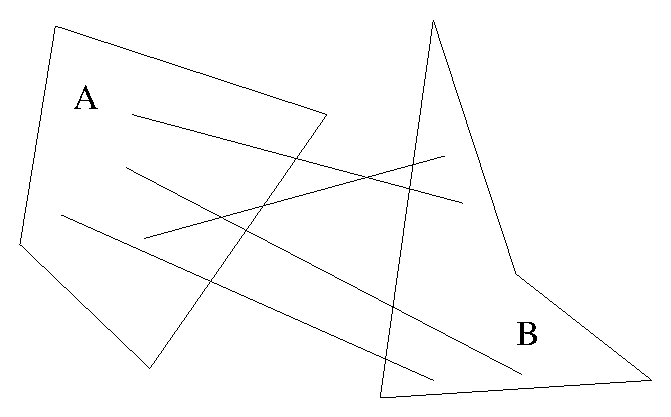
\includegraphics[width=7.5cm]{VignetteDir/graphics/integral_geom_1.eps}}
  \subfigure[Consider all the pairs of points separated by 
  the same vector $t$ ($t$ is in bold on the figure). For a given $t$, 
  $x\in A$ and $x+t\in B$, if and only if  $x\in
  A\cap\left(B-t\right)$ (such $x$ and $x+t$ are joined here by blue
  segments; $A\cap\left(B-t\right)$ is represented by 
 the blue area).]{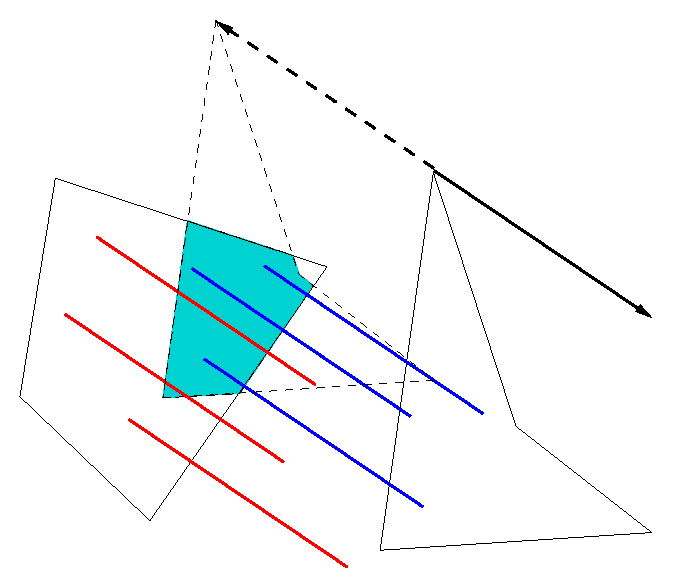
\includegraphics[width=7.5cm]{./VignetteDir/graphics/integral_geom_2.eps}}
  \caption{The quantity of particles from a polygon $A$
to a polygon $B$ is computed
by integrating the individual dispersal function
over all pairs of points $(x,y) \in A\times B$.
These pairs are represented here by segments.}
    \label{fig:int:geom:1}
\end{figure}

\medskip

Rather than scrolling through the pairs of points by choosing 
each member independently in  $A$ and $B$,
it is worth considering the pairs separated by the same vectors.
The dispersal function is constant on such subsets  of the pairs of
points.

\medskip
With the variable change $(x,y)\rightarrow (x,t=y-x)$, the set
\begin{equation*}
  \left\{y-x|x\in A, y\in B\right\}
\end{equation*}
can be written  $\check{A}\oplus B$ where $\check{A}=-A$
and $\oplus$ stands for the Minkowski sum.
The Minkowski sum of two sets $A$ and $B$ is simply the set obtained
by addition of the points of $A$ and $B$ (see
Fig.~\ref{fig:minkowski}). On the other hand, for each
vector $t\in \check{A}\oplus B$: 
\begin{equation*}
  x\in A, y=x+t\in B \Leftrightarrow x\in A\cap\left(B-t\right) 
\end{equation*}

\begin{figure}[htbp]
  \begin{center}
    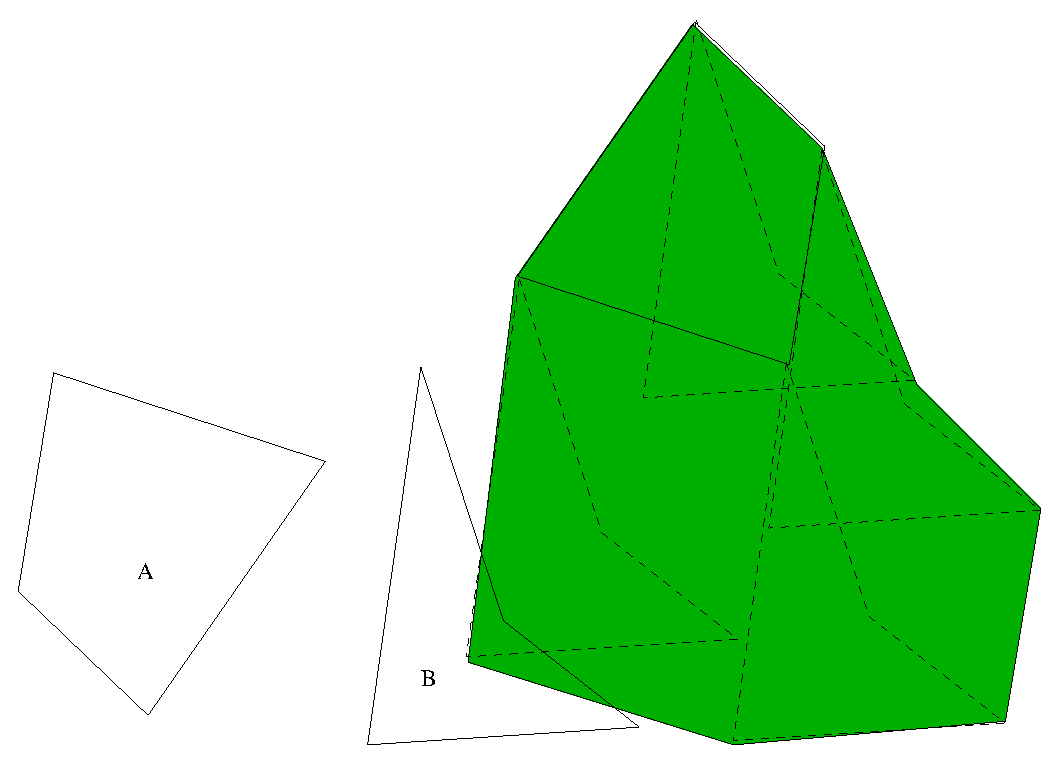
\includegraphics[width=10cm]{./VignetteDir/graphics/integral_geom_4.eps}
    \caption{The set of points $t=y-x$, where $x\in A$ and 
$y\in B$, is written $\check{A}\oplus B$. 
It is the set of points
covered by $B$ when the vertex $o$ is moved inside $\check{A}$.
Here, to simplify, the origin of the plan $o$ is
located on a vertex of  $B$.}
    \label{fig:minkowski}
  \end{center}
\end{figure}

Now, we can rewrite the integral $\A$ 
defined by the equation~\eqref{eq:def:A}:
\begin{eqnarray}
  \A &=& \int_{\check{A}\oplus B}\int_{A\cap \left(B-t\right)} 
  \phi(t) \,dx\,dt
\end{eqnarray}
as:
\begin{eqnarray}
  \A & = & \int_{\check{A}\oplus B}\int_{A\cap \left(B-t\right)} 
  \,dx\, \phi(t) \,dt.
\end{eqnarray}

The integral in $x$ is simply the area of $A\cap
\left(B-t\right)$, so:
\begin{equation}
  \label{lastexpression}
  \A = \int_{\check{A}\oplus B} \aire(A\,\cap\,(B-t)) \,\phi(t)
  \,dt 
\end{equation}

The computation of one of the two integrals has been replaced
by the computation of an area and of an intersection, the intersection
of  $A$ and a translation of $B$.
The calculation of~\eqref{lastexpression} has
proven to be faster than the one of~\eqref{eq:def:A}
\footnote{Time comparisons have been made by using the 
integration subroutines of the NAG~\cite{NAG} library,
D01FCF (adaptive integration, i.e where the evaluation 
spots depend
on the integrand), and  D01GCG (Korobov-Conroy method) 
on  real and simulated fields.}
So, it is the formula implemented in \verb+CaliFloPP+.


%%% Local Variables: 
%%% mode: latex
%%% TeX-master: t
%%% End: 


 

\chapter{Geometric Computation}
\label{sec:geom:algo}

In order to compute numerically the two-dimensional
integral~\eqref{lastexpression}, one must compute the area of the
intersection $\aire(A\,\cap\,(B-t))$ for different values of
$t\in\check{A}\oplus B$ (domain of integration) where $A$ and $B$ are
polygons. Note that $A$ and $B$ are not necessarily convex.
Computations of polygonal areas, intersections and Minkowski sums are
known problems in \emph{computational geometry}. The
textbook~\cite{ORourke:1998} is a rather nice introduction to that
topic. Most algorithms briefly described below are provided
there. Note that this chapter is only devoted to the computation of
the geometric features involved in the
integral~\eqref{lastexpression}. The problem of numerical integration
is treated in Chapter~\ref{sec:integrale}.

The intersection $A\,\cap\,(B-t)$ is a polygon. The computation of the
area of a polygon is straightforward, see
Section~\ref{sec:calcul:aire} for the case when the polygon is convex.

The computation of the intersection $A\,\cap\,(B-t)$ is easy when both
$A$ and $B$ are convex, see Section~\ref{sec:calcul:intersection}.
When either $A$ or $B$ is not convex, the intersection may be
complicated. In particular, it may not be connected.

The computation of the Minkowski sum $\check{A}\oplus B$ is rather
easy if $A$ or $B$ are convex, see Section~\ref{sec:calcul:somme}.

Hence the computation of the integral~\eqref{lastexpression} is easy
when both $A$ and $B$ are convex. This is why we propose to first
decompose $A$ and $B$ as unions of convex polygons:
\begin{equation}
  \label{eq:convex:decomp:A:B}
  A = \bigcup_{i=1}^n A_i,\qquad B = \bigcup_{j=1}^m B_j,
\end{equation}
where the areas of $A_{i}\cap A_{i'}$, respectively $B_{j}\cap
B_{j'}$, are equal to $0$ whenever $i\neq i'$, respectively $j\neq
j'$. An algorithm for computing such a decomposition is
described in Section~\ref{sec:decompo}. It is easy to check that the
integral~\eqref{lastexpression} can be written as:
\begin{equation}
  \label{eq:integral:decomposition}
  \int_{\check{A}\oplus B} \aire(A\,\cap\,(B-t)) \,\phi(t)
  \,dt =
  \sum_{i=1}^n \sum_{j=1}^m
  \int_{\check{A}_i\oplus B_j} \aire(A_i\,\cap\,(B_j-t)) \,\phi(t)
  \,dt.
\end{equation}
Based on the algorithm for decomposing polygons into convex ones and
tools for computing numerically the integral~\eqref{lastexpression}
for any pair $(A,B)$ of convex polygons (see Chapter
\ref{sec:integrale}), the integral~\eqref{lastexpression} for an
arbitrary pair of polygons can be computed using
Algorithm~\ref{algo:int:any:pair}.

% \begin{algorithm}
%   \caption{Integral computation for an arbitrary pair of polygons}
%   \label{algointanypair}
%   \begin{algorithmic}[1]
%     \REQUIRE Two polygons $A$ and $B$.
%     \ENSURE Computation of $\aire(A\,\cap\,(B-t))$ for an arbitrary vector 
%     $t$.
%     \STATE Compute convex polygons $A_1,\ldots,A_n$ such that
%     $A=\cup_{i=1}^n A_i$ and such that $\aire(A_{i}\cap A_{i'})=0$ if
%     $i\ne i'$.
%     \STATE Compute convex polygons $B_1,\ldots,B_m$ such that
%     $B=\cup_{j=1}^m B_j$ and such that $\aire(B_{j}\cap B_{j'})=0$ if
%     $j\ne j'$.
%     \STATE $\A=0$
%     \FORALL{$i=1,\ldots,n$}
%     \FORALL{$j=1,\ldots,m$}
%     \STATE Increment $\A$ by
%     $$\int_{\check{A}_i\oplus B_j} \aire(A_i\,\cap\,(B_j-t))\,
%     \phi(t)\,dt.$$ 
%     \ENDFOR
%     \ENDFOR
%   \end{algorithmic}
% \end{algorithm}

\begin{algorithm}
  \caption{Integral computation for an arbitrary pair of polygons}
  \label{algo:int:any:pair}
  \KwData{Two polygons $A$ and $B$, a dispersal function $\phi$.}
  \KwResult{Computation of $\aire(A\,\cap\,(B-t))$ for an arbitrary vector 
    $t$.}
  Compute convex polygons $A_1,\ldots,A_n$ such that
  $A=\bigcup_{i=1}^n A_i$ and such that $\aire(A_{i}\cap A_{i'})=0$ if
  $i\ne i'$\;
  Compute convex polygons $B_1,\ldots,B_m$ such that
  $B=\bigcup_{j=1}^m B_j$ and such that $\aire(B_{j}\cap B_{j'})=0$ if
  $j\ne j'$\;
  $\A=0$\;
  \For{$i=1,\ldots,n$}{
    \For{$j=1,\ldots,m$}{
      Increment $\A$ by
      $$\int_{\check{A}_i\oplus B_j} \aire(A_i\,\cap\,(B_j-t))\,
      \phi(t)\,dt;$$
    }
  }
\end{algorithm}

Below, convex polygons are represented as sequences of vertices
labeled counterclockwise:
\newline
$(v_0,\ldots,v_{n-1})$.
Many computations
involve cycling over vertices. Hence it is convenient
to use the convention $v_n=v_0$. All edges can be represented as
$e_i=(v_i,v_{i+1})$, $i=0,\ldots,n-1$.

% \section{Tester si un point est à l'intérieur d'un polygone}
% \label{sec:interieur}

% Un point est à
% l'intérieur d'un polygone convexe si et seulement si  ce point est toujours 
% à gauche lorsque l'on parcourt le périmètre du polygone.
% Voir Fig ~\ref{figinpoly}.
% \begin{figure}[htbp]
%   \begin{center}
%   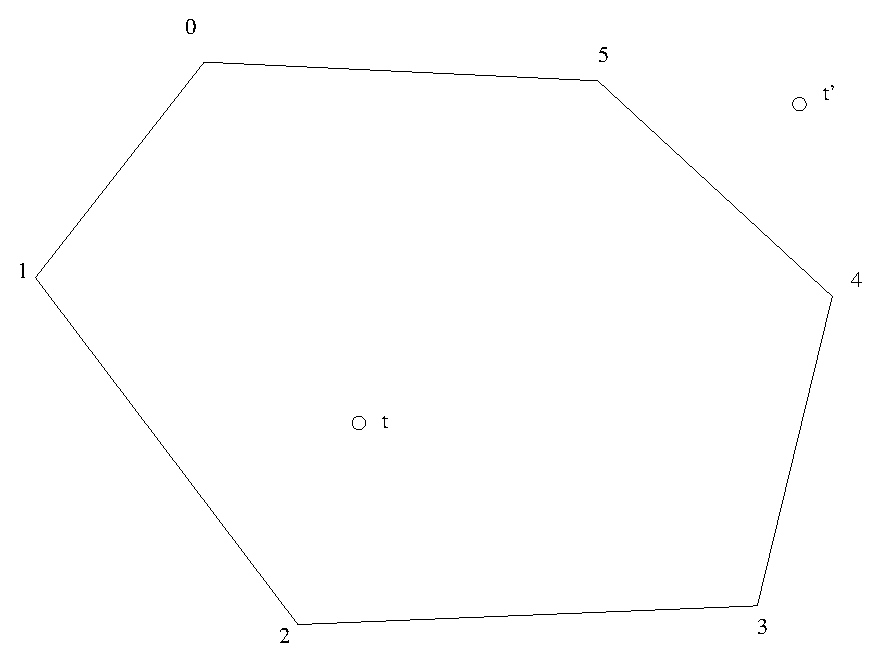
\includegraphics[width=9cm]{./graphics/inpoly.eps}
%   \end{center}
%   \caption{Tester si un point est à l'intérieur d'un polygone:
% le point $t'$ n'est pas à gauche de l'arête 4-5: il n'est donc pas dans
% le polygone, à l'inverse du point $t$ qui est à gauche de toutes les arêtes.}\label{figinpoly}
% \end{figure}

% \medskip
% {\small
% Remarque:
% Une méthode générale,  valide même
% pour un polygone non convexe, est basée sur le même principe.
% On calcule le nombre de points d'intersection d'une droite passant par
% le point avec le polygone. On peut prendre, par exemple, une droite
% horizontale. Si le nombre d'intersections à gauche du point testé est
% impair, le point est à l'intérieur.
% }

\section{Area of a convex polygon}
\label{sec:calcul:aire}

%% Remarques :
%% -----------
%%
%% - Il vaudrait mieux utiliser la formule générale. Pas tellement par
%%   souci d'efficacité, mais parce que le code serait plus clair.
%% - Les fonctions pour calculer des aires de triangles sont Area2
%%   (calcul sur des flottants) , Area2i (calcul sur des entiers). En
%%   fait, ces fonctions calculent le double de l'aire. En effet, ce
%%   résultat est entier si les coordonnées le sont aussi. Ce
%%   qui est assez bizarre, c'est que Area2i fait le calcul en
%%   flottants puis une conversion en entier. Ca permet d'avoir moins
%%   d'overflow. Mais il faut faire attention si Area2i n'est pas
%%   utilisé pour tester des prédicats (du genre C est à gauche de AB)
%%   car alors le résultat peut ne pas être correct.
%% - La fonction area_polygon_2 calcule le double de l'aire d'un
%%   polygone. Il faudrait changer le nom de l'argument et supprimer
%%   les sorties de débogage.

A convex polygon can be decomposed into triangles, see
Figure~\ref{figairepoly}. Thus its area is
the sum of its triangles areas. Each of them is computed using the
following formula
\begin{equation}
  \label{eq:triangle:area}
  \frac{1}{2}(x_B - x_A)(y_C - y_A) - (x_C - x_A)(y_B - y_A),
\end{equation}
where $A$, $B$ and $C$ are the triangle vertices and the $x$'s and
$y$'s are Cartesian coordinates. Equation~\eqref{eq:triangle:area}
yields a signed area. It is positive if $A$, $B$ and $C$ are ordered
counterclockwise, otherwise it is negative. The final result is exact
if the coordinates are integers.  The computing time depends on the
number of polygon vertices. Algorithm~\ref{algo:area} describes the
whole procedure. Note that if the polygon vertices are numbered
counterclockwise then the triangle vertices are also numbered
counterclockwise.
\begin{algorithm}[tbph]
  \caption{Area of a convex polygon. Triangle areas are computed
    using Equation~\eqref{eq:triangle:area}.}
  \label{algo:area}
  \KwData{Convex polygon with vertices (numbered counterclockwise)
    $v_0,\ldots,v_{n-1}$.}
  \KwResult{Area of the polygon.}
  $a=0$\;
  \For{$i=1,\ldots,n-2$}{
    $a=a+\aire(\text{triangle } v_{0},v_i,v_{i+1})$\;
  }
\end{algorithm}
%%
\begin{figure}[tbph]
  \begin{center}
    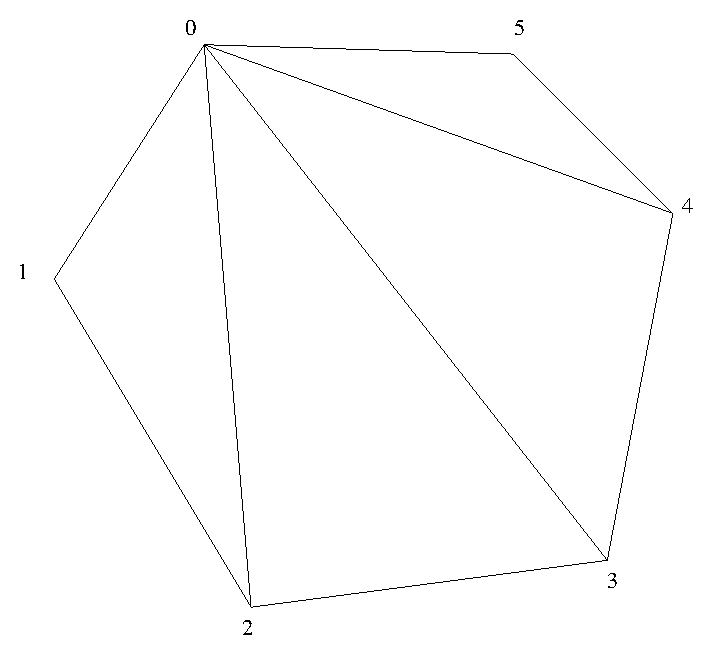
\includegraphics[width=9cm]{./VignetteDir/graphics/airepoly.eps}
    \caption{Decomposition of a convex polygon into triangles. An
      arbitrary vertex is connected to all non adjacent vertices.}
    \label{figairepoly}
  \end{center}
\end{figure}
%%

For area computation convexity is not an issue. The area of an
arbitrary polygon is also easy to compute. If
$(x_0,y_0),\ldots,(x_{n-1},y_{n-1})$ are the Cartesian coordinates of
the vertices (numbered counterclockwise) of a polygon, its area is
equal to
\begin{equation}
  \label{eq:area:any:polygon}
  \frac{1}{2}\sum_{i=1}^{n-1} (x_i+x_{i+1})(y_{i+1}-y_i).
\end{equation}

\section{Intersection of two convex polygons}
\label{sec:calcul:intersection}

%% Remarque : on peut avoir des problèmes numériques. Par exemple, on
%% peut tester a meets b positivement et avoir un pb avec le calcul de
%% l'intersection de a et b. Le test intersection de a et de b =
%% premier sommet du plygone résultat peut aussi être problématique (?).

Here we focus on the case when the boundaries of the two convex
polygons $P$ and $Q$ meet each other: the cases where the intersection
is void or where one polygon is included in the other one are not
considered.

The intersection $P\cap Q$ is a convex polygon whose vertices are
vertices of $P$ or vertices of $Q$ or intersection of edges of $P$
with edges of $Q$. The intersection can be computed using the
algorithm described in \cite[Section 7.6]{ORourke:1998}. Two orientated
edges $a\subset P$ and $b\subset Q$ are chosen. The edges $a$ and $b$
are advanced so  that all the vertices of $P\cap Q$
can be detected and recorded, see
Algorithm~\ref{algo:intersection:convex:poly}. Note that special cases
are not treated: the algorithm is valid if $P$ and $Q$ are in general
relative position, i.e.\ their boundaries cross only at the interior
of edges. Also the implementation of this algorithm requires some
further low-level functions:
\begin{itemize}
\item Test whether two segments meet.
\item Compute the intersection of two segments.
\item The advancing rule can be reformulated and requires only the
  computation of signed areas see \cite[Section 7.6]{ORourke:1998} for
  further details.
\end{itemize}

\begin{algorithm}[tbph]
  \caption{Intersection of two convex polygons}
  \label{algo:intersection:convex:poly}
  \KwData{Two convex polygons $P$ and $Q$}
  \KwResult{Computation of $P\,\cap\,Q$.}
  Choose an edge $a$ of $P$ and an edge $b$ of $Q$\;
  $R=\emptyset$\;
  \Repeat{both $a$ and $b$ cycle along $P$ and $Q$ boundaries}{
    \eIf{$a$ meets $b$}{
      \eIf{$a\cap b$ coincides with the first vertex of $R$}{
        Terminate\;
      }{
        Add $a\cap b$ to $R$\;
      }
      Advance either $a$ or $b$\;
    }{
      \eIf{One edge points toward the line containing the
        other}{
        Advance it\;
      }{
        \eIf{One edge is on the right-hand side of the other}{
          Advance it\;
        }{
          Advance either $a$ or $b$\;
        }
      }
    }
  }
\end{algorithm}

\section{Minkowski sum of convex polygons}
\label{sec:calcul:somme}

Let $P$ and $Q$ be two convex polygons. An algorithm for computing the
so-called convolution of $P$ and $Q$ is described in~\cite[Section
8.4]{ORourke:1998}. When both $P$ and $Q$ are convex, the convolution
is equivalent to the Minkowski sum. The computation of the convolution
is based on the \emph{star diagram} of $P$ and $Q$ edges. For any edge
$e$ of $P$ Let $\alpha(e)\in[0,2\pi)$ be the angle of $e$ with an
arbitrary axis. The star diagram is a polar representation of the
$\alpha's$. The Algorithm~\ref{algo:minkowski} shows how to compute
the Minkowski sum from the star diagram. Due to the convexity
assumption, $\alpha$ is increasing on the set of edges of a polygon if
the reference axis is parallel to its first edge.
\begin{algorithm}[tbph]
  \caption{Minkowski sum of two convex polygons.}
  \label{algo:minkowski}
  \KwData{Two convex polygons $P$ and $Q$.}
  \KwResult{The Minkowski sum $P\oplus Q$.}
  \tcp{Star diagram}
  Compute $\alpha$ for all edges of $P$ and $Q$ taking as the
  reference axis a line parallel to the first edge of $P$\;
  Sort the $\alpha$'s: $\alpha_k$, $k=0,\ldots,n+m-1$ where $n$ is the
  number of $P$-vertices and $m$ is the number of $Q$-vertices\;
  $R=\{\text{first vertex of }P\}$\;
  \For{$k=0,\ldots,n+m-1$}{
    Add to $R$ the latter vertex of $R$ translated by $\vec{e}$ where $e$ is
    the edge associated with $\alpha_k$\;
}
\end{algorithm}

\section{Convex partitioning of a polygon }
\label{sec:decompo}

In order to implement Algorithm~\ref{algo:int:any:pair}, one needs to
decompose an arbitrary polygon into convex polygons. The decomposition
algorithm is three-step:
\begin{enumerate}
\item The polygon $P$ is triangulated using an ear removal algorithm,
  see e.g.\ \cite[Section 1.6]{ORourke:1998}.
\item Essential diagonals of the triangulation are identified.
\item The convex subpolygons are created.
\end{enumerate}
An internal (resp.\ external) diagonal is a segment joining two
vertices which is contained in (resp.\ lies outside) the polygon. An
ear is a triangle inside the polygon whose vertices are three
consecutive vertices $a,b,c$ of the polygon, i.e. $ac$ is an internal
diagonal. 

The triangulation algorithm, see Algorithm~\ref{algo:triangulation},
consists in successive ear removals. In order to test whether a vertex
$v_i$ is an ear tip, one tests whether $v_{i-1}v_{i+1}$ is an internal
diagonal. The latter test is decomposed into two steps: first test
whether $v_{i-1}v_{i+1}$ is a diagonal (internal or external), second
test if $v_{i-1}v_{i+1}$ is internal. The first test involves edge
intersection tests (loop along the edges). For the second test, one
has to consider two cases:  $v_{i}$ is convex or reflex. The second
test requires only computation of signed areas.


The triangulation yields internal diagonals (inner edges of the
triangulation). 
A non-essential diagonal divides two adjacent cells
whose union is still convex. It is easy to check that a diagonal is
non-essential if both  its ends are convex. 



\begin{algorithm}[tbph]
  \caption{Triangulation of a polygon.}
  \label{algo:triangulation}
  \KwData{A polygon $P$ with vertices $v_0,\ldots,v_{n-1}$.}
  \KwResult{A triangulation of $P$}
  \tcp{Find ear tips}
  \For{$i=0,\ldots,n-1$}{
    \If{$v_{i-1}v_{i+1}$ is an internal diagonal}{
      Set $v_i$ as an ear tip\;
    }
  }
  $T=\emptyset$\;
  $v=$ first vertex of $P$\;
  \While{$P$ has more than $3$ vertices}{
    \If{$v$ is an ear tip}{
      Add to $T$ the triangle $uvw$ where $u$ is the vertex previous
      to $v$ and $w$ is the vertex next to $v$\;
      \tcp{Update ear tip status of $u$ and $w$}
      \If{the vertices before and after $u$ form a diagonal}{
        Set $u$ as an ear tip\;
      }
      \If{the vertices before and after $v$ form a diagonal}{
        Set $v$ as an ear tip\;
      }
      Remove $v$ from $P$\;
    }
    Advance $v$\;
  }
\end{algorithm}

The last step is to split the polygon according to computed essential
diagonals, see Algorithm~\ref{algo:split}.

\begin{algorithm}
  \caption{Creation of convex polygons from the essential diagonals}

  \label{algo:split}
\KwData{A nonconvex polygon: its $nvertices$ vertices and $ndiagonals$
diagonals; the essential diagonals are marked.
The sides of the polygon are essential diagonals.}
\KwResult{The $np$ convex subpolygons: their vertices are stored
  anticlockwise in $polyg$.}
$np=0$\\
\While{there is an essential diagonal}
{ $(v_a,v_b)$ = any  essential diagonal\\
$start = va$\\
\While{ $vb != start$}
{store $(v_a,v_b)$ into $polyg[np]$\\
mark $(v_a,v_b)$ non-essential\\
\tcp{Determine the following diagonal:}
$(v_b,v_c)$ is the diagonal starting from $v_b$ and such as the angle
$(v_a,v_b,v_c)$ is minimum\\
$v_a=v_b; v_b=v_c$
}
$np=np+1$
}
\end{algorithm}




\chapter{Two-dimensional Numerical Integration}
\label{sec:integrale}

This chapter is devoted to the numerical computation of integrals of
the type
\begin{equation}
  \label{eq:integral:to:compute}
  \int_{\check{A}\oplus B} \aire(A\,\cap\,(B-t)) \,\phi(t)
  \,dt,
\end{equation}
where $A$ and $B$ are bounded polygons and $\phi$ is an arbitrary
integrable dispersal function. As seen in
Chapter~\ref{sec:geom:algo}, without loss of generality we can focus
on the case when both $A$ and $B$ are convex.

We will start by preliminary remarks concerning the smoothness of the
integrand. Then we will discuss two methods for numerical integration:
\begin{itemize}
\item A simple randomized discretization of the integral;
\item An adaptive cubature method.
\end{itemize}

The first method, described in Section~\ref{sec:integration:autres},
combines simple discretization and Monte-Carlo techniques. This method
is quite robust (convergence even for non-smooth integrands). It
yields unbiased estimates and it is able to assess its precision.
However it may be slow compared to other methods.

The second method consists of an adaptive cubature. First, the domain of
integration (a convex polygon) is triangulated. Then the integral over
each triangle is approximated using the adaptive cubature method
proposed by Berntsen and Espelid~\cite{berntsen_espelid}. The
convergence of this method depends on the smoothness of the
integrand. It may fail to converge if the integrand cannot be
approximated locally by a polynomial. Some basic results about the
smoothness of the integrand in Equation~\eqref{eq:integral:to:compute}
are stated in Section~\ref{sec:regularite}. Details about the
adaptive cubature method are provided in Section~\ref{sec:cubature}.


\section{Smoothness of the integrand}
\label{sec:regularite}

The integrand in Equation~\eqref{eq:integral:to:compute} is the
product of two functions:
\begin{equation*}
  \aire(A\,\cap\,(B-t)) \text{ and } \phi(t).
\end{equation*}
The function $t\mapsto\aire(A\,\cap\,(B-t))$ is a piecewise linear
function. Its support $\check{A}\oplus B$ can be split by line
segments obtained by adding edges of $\check{A}$ and edges of $B$, see
Figure~\ref{fig:partition:minkowski}. Inside each cell of this
partition, $t\mapsto\aire(A\,\cap\,(B-t))$ behaves linearly. The
differential $t\mapsto\aire(A\,\cap\,(B-t))$ is not continuous along
the network of cell boundaries.
\begin{figure}[htbp]
  \centering
  \input{VignetteDir/graphics/div_minkowski_convexe.pstex_t}
  \caption{Partitionning of the Minkowski sum of two convex polygons
    $A$ and $B$ according to their edges.}
  \label{fig:partition:minkowski}
\end{figure}

The smoothness of the whole integrand also depends on the smoothness
of the dispersal function $\phi$. For instance, the dispersal
function given in Equation~\eqref{eq:dispersion:colbach} is infinitely
continuously differentiable except at the origin where it is not twice
differentiable.  Then the whole integrand is infinitely continuously
differentiable except along the cell boundaries in the partition of
the Minkowski sum where it is not differentiable and at the origin
where it is not twice differentiable. Another example: the dispersal
function given in Equation~\eqref{eq:dispersion:klein} is not
differentiable at the origin and it is not twice differentiable along
a circle with radius $1.5$ meter centered at the origin. Then the
whole integrand is not differentiable neither at the origin nor along
the cell boundaries and it is not twice differentiable along the circle.


\section{Method based on grids of points}
\label{sec:integration:autres}

A simple and intuitive method to perform numerical integration consists
of evaluating the integrand over a regular grid of points. The integral
is then approximated by summing the integrand over the grid points, and
by multiplying the result by the volume of each cell in the grid.
Provided the grid position is randomised, this method yields an unbiased
estimate of the integral. In addition, it can be repeated
several times, with grid positions randomised independently. The
integral is then estimated by the mean over the replicated grids. Replications
increase precision but also allow the standard error to be estimated. 

To simplify, this method will be called \textbf{the grid method} in the
sequel. In \verb+CaliFloPP+, the distances between the nodes of the grids are the same
for all grids and they are chosen by the user. The number of
replications is also set by the user.

\label{grille}
Let $A$ and $B$ be two polygons. The main steps are~:
\begin{enumerate}
\item
calculation of the Minkowski sum $\check{A}\oplus B$~;
\item
determination of the smallest rectangle which includes the Minkowski sum
and whose sides are parallel to the axes (see Fig.~\ref{integrale})~;
\item
integration over this rectangle, with the integrand multiplied by a coefficient 
$w$ equal to~1 if the point is in the Minkowski sum, to~0 otherwise.
\end{enumerate}

Integration is performed as mentioned above, using several grids of
points with the following properties~:
\begin{itemize}
\item all grids have the same $x$ and $y$ lags between adjacent nodes, chosen
  by the user~;
\item each grid is positioned randomly on the integration area, by
  shifting it randomly relatively to the origin. The shifting is
  determined by pseudo-random numbers from the uniform distributions
  over the intervals $[0, p_x]$ and $[0, p_y]$, where $p_x$ and $p_y$
  denote the $x$ and $y$ lags between adjacent grid nodes.
\end{itemize}
The integral is estimated by the mean integral over the replicated grids.

\subsection{Additional results}
\begin{itemize}
\item
\textbf{Standard deviation}

The \texttt{standard deviation} is defined as~: 
\begin{equation}
\mathrm{sd} = \frac{ \sqrt{\sum_{i=1}^{r} (a_{i} - a_{\bullet})^2}} {
  r-1}
\end{equation}
where  $a_{i}$ is the integral value calculated by replication $i$,
and $r$ the number of grid replications.

\item\textbf{Coefficient de variation} 

The \texttt{coefficient de variation} is defined as~: 
\begin{equation}
\mathrm{CV} = \frac{\mathrm{sd}}{a_{\bullet}}
\end{equation}


\item
\textbf{Precision and confidence intervals}
\label{it:gridprec}

Precision and confidence intervals can be calculated by the user
from the replications results.
For example, when the number of replications is large enough and  the
distributions are symmetric, they can be calculated from the quantile
of the Student distribution.
The half-range $\mathrm{hr}$ of the confidence
interval, or the absolute precision, is then defined as~:
\begin{equation}
\mathrm{hr} =  \mathrm{sd} \times \frac{\mathrm{qt}(r-1, p)}{\sqrt{r}}
\end{equation}
where  $\mathrm{qt}(n,p)$ is the quantile for probability $p$ of the Student
distribution with $n$ degrees of freedom.
The relative precision is $\frac{hr}{a_{\bullet}}$.
\end{itemize}


\begin{figure}[htbp]
  \begin{center}
  \includegraphics[width=9cm]{VignetteDir/graphics/integrale.eps}
  \end{center}
  \caption{Minimal rectangle including the Minkowski sum and grid of
    points before random shifting}
  \label{integrale}
\end{figure}



\section{Adaptive cubature method}
\label{sec:cubature}

The cubature method over triangles DCUTRI \cite{berntsen_espelid} uses
an integration rule of degree $27$ based on $37$ points. Using
estimates of approximation errors, triangles are iteratively split
into subtriangles until a nominal error is reached. At each iteration
the triangle with the largest error is selected for further splitting.
The procedure is expected to converge if the integrand is smooth
enough inside each triangle. For instance, if the dispersal function
is singular at the origin and if the domain of integration
$\check{A}\oplus B$ contains the origin, one expects a quicker
convergence when the origin is a vertex of the triangulation. Hence
(see Figure~\ref{fig:triangulation:minkowski}):
\begin{itemize}
\item if $\check{A}\oplus B$ does not contain the origin, it is
  triangulated from an arbitrary vertex,
\item if $\check{A}\oplus B$ contains the origin $O$, it is
  triangulated from $O$.
\end{itemize}

\begin{figure}[htbp]
  \centering
  \input{VignetteDir/graphics/triangulation_minkowski.pstex_t}
  \caption{Triangulation of the Minkowski sum of two convex polygons
    $A$ and $B$. If $A$ and $B$ are disjoint (top), the Minkowski sum
    $\check{A}\oplus B$ does not contain the origin and is
    triangulated from an arbitrary vertex. If $A$ and $B$ share a
    common edge (middle) or if $A=B$ (bottom), the Minkowski sum
    $\check{A}\oplus B$ contains the origin $O$ and is
    triangulated from $O$.}
  \label{fig:triangulation:minkowski}
\end{figure}

A further refinement is to avoid to integrate over areas where the
dispersal function is considered as negligible that is below a chosen
threshold $r_\text{max}$. Note that whenever the dispersal function
is non-negative and tends to $0$ at infinity, it can be considered in
practice as null when it is less than the smallest positive number
greater than zero for the used type of number. Thus instead of
integrating over the whole Minkowski sum $\check{A}\oplus B$, one may
integrate only on its intersection with a disc centered at the origin
and with radius $r_\text{max}$. In practice it is simpler to replace
the disc by a regular polygon e.g.\ an octogon containing it, see
Figure~\ref{fig:reduc:minkowski}. Hence integration is still performed
on a convex polygon.
\begin{figure}[htbp]
  \centering
  \input{VignetteDir/graphics/reduc_minkowski.pstex_t}
  \caption{Reduction of the domain of integration. Beyond
    $r_\text{max}$ the dispersal function is considered as
    negligible. The integral is computed only over the intersection of
    $\check{A}\oplus B$ and an octogon (blue solid line) containing
    the disc centered at the origin with radius $r_\text{max}$ (blue
    dash line). Top: the Minkowsi sum $\check{A}\oplus B$ does not
    contain the origin
. Bottom: the Minkowski sum contains the origin.}
  \label{fig:reduc:minkowski}
\end{figure}

%%% On n'a plus besoin des graphiques octo.eps et octo0.eps




%%% Local Variables: 
%%% mode: latex
%%% TeX-master: "../manotice"
%%% End: 

\part{Example}
\label{sec:ex}

\section{Introduction}
In this Section, we analyze the behavior
of the grid and  cubature methods on a real landscape.
First, we compare the results calculated with different 
parameterisations 
of each  method; then,
 the two methods are compared.

\subsection{Data}
The data are 66 polygons extracted from
the ORTHO demo, a IGN\footnote{Institut Géographique National:
  \href{http://www.ign.fr/rubrique.asp?rbr\_id=1619}
{http://www.ign.fr/rubrique.asp?rbr\_id=1619}} data base
, see~Fig.~\ref{fig:parcelle}.
\begin{figure}
  \begin{center}
    \includegraphics[angle=-90, width=15cm]{./VignetteDir/graphics/parcelles.ps}
  \end{center}
\caption{Example of 66  polygons extracted from the ORTHO IGN data base. Unit is meter.}\label{fig:parcelle}
\end{figure}
To illustrate  contrasted situations,
five pairs of polygons are treated:
\begin{itemize}
\item
\textbf{(1,1)}: two identical convex polygons,
\item
\textbf{(14,14)}: two identical non-convex polygons,
\item
\textbf{(11,12)}: two convex polygons next to each other,
\item
\textbf{(56,57 )}: two polygons next to each other, one  convex, the
other non-convex,
\item
\textbf{(4,4)}: two identical very irregular polygons.
\end{itemize}
The individual dispersal function is
the oilseed rape pollen dispersal function
defined in~Section~\ref{pollen:funct}.


\section{Influence of the parameterisation in the grid method}


In the grid method, two parameters must be chosen
according to the user's needs:
 the number of
replications and  the grid step.

\subsection{Influence of the number of replications}

To compare the results calculated with different numbers of
replications, 
four values were successively applied:
$r=$ 5, 10, 15, 20. The grid step was constant and equal to 1~m
for both axes.

The results\footnote{Results are dependent on the random numbers generator; so,
actual values may be slightly different.} 
are given in~Table~\ref{array:nr}.
They are:
the evaluated mean flow ($\widehat{\A}$),
the standard deviation ($\widehat\sigma$),
 the coefficient of variation ($\widehat\sigma/\widehat{\A}$)
and the execution time\footnote{
Execution times depend on the material context.
They have been observed here on a Dell Biprocessor, in shared mode
and 3,2GhZ.}.
We can notice that 
the execution times are the
longer as the polygons are the more irregular:
calculation is faster on convex polygons 
(1$\leftrightarrow$1, 11$\leftrightarrow$12) than on non convex ones
(14$\leftrightarrow$14, 56$\leftrightarrow$57)
and very much longer on irregular polygons (4$\leftrightarrow$4).


\begin{table}
\footnotesize
\caption{\label{array:nr} Grid results  with different
  numbers of replications ($r$) and grid step equal to 1~m.}
\begin{center}
\begin{tabular}{|p{1.5cm}|p{1.5cm}|p{1.5cm}|p{1.5cm}|p{1.5cm}|p{1.2cm}|}
\hline
\textbf{Polygons} & 
$r$ & $\widehat{\A}$ &
$\widehat\sigma$ & $\widehat\sigma/\widehat{\A}\times$100  & $Times$
 \\ \hline
1$\leftrightarrow$1 & 5 & 12222.2  & 234.6 & 1.88 & 3.5\\
 & 10   & 12282.5  & 217.7 & 1.77 &  7.0 \\
 & 15 & 12238.8  &  204.1 & 1.66 & 10.5 \\
 & 20 &  12247.7  &  220.9 & 1.80 & 14.1
 \\ \hline
14$\leftrightarrow$14&  5 &  23542.1  & 461.6   & 1.96 & 31.9 \\
 &  10   &  23359.0   & 391.1 & 1.67 & 63.7\\
&  15 & 23411  &  344.4  & 1.47 & 95.3\\
& 20 &  23413.3  & 332.4 & 1.41 & 126.7
 \\ \hline
11$\leftrightarrow$12 &  5 & 164.5  & 2.4 & 1.48 & 7.0 \\
 &  10   & 166.1  & 3.1 & 1.89 & 14.0\\
&  15 & 167.3  & 3.1 & 1.85 & 21.1 \\
& 20 & 167.2  & 3.1 & 1.84 & 27.9
 \\ \hline
56$\leftrightarrow$57 &  5 & 132.5  & 2.0 & 1.51 & 5.9 \\
&  10   & 133.0  & 2.2 & 1.70 & 11.7\\
& 15 &  132.5  & 2.1 & 1.62 &  17.6\\
& 20 & 132.8  & 1.9 & 1.49 & 23.4
 \\ \hline
4$\leftrightarrow$4 &  5 & 14610.1  & 72.3 & 0.5 & 45.7 \\
 & 10   & 14570.9  & 91.5 & 0.62 & 90.7\\
&  15 & 14617.7  & 155.2 & 1.06 & 136.7\\
& 20 &14631.5  & 151.5 & 1.03 & 181.2
 \\ \hline
\end{tabular}
\end{center}
\normalsize
\end{table}



\subsection{Influence of the grid step}


To compare the results calculated with different grid steps, 
four values were tried successively:
$step=$~0.25~m,~0.5~m,~0.75~m~and~1~m.
The number of replications, $r$, is set to 10.

The results are displayed in Table~\ref{array:step}.
As expected, 
the  times  increase
 as the steps become smaller.

\begin{table}
\footnotesize
\caption{\label{array:step} Grid results  with different steps
($r=10$);}
\begin{center}
\begin{tabular}{|p{1.5cm}|p{1.5cm}|p{1.5cm}|p{1.5cm}|p{1cm}|p{1.5cm}|}
\hline
\textbf{Polygons} & $step$ & $\widehat{\A}$ &
$\widehat\sigma$ & $\widehat\sigma/\widehat{\A}\times$100  & $Times$
 \\ \hline
1$\leftrightarrow$1  
 & 1   & 12282.5  & 217.7 & 1.77 &  7.0\\
& 0.75 & 12196.9  & 27.3 & 0.22 & 12.6 \\
& 0.5 & 12277  &  32.8 & 0.26 & 28.5\\
& 0.25 & 12273.8   & 4.08 & 0.03 & 111.5\\
\hline
14$\leftrightarrow$14
 &  1   & 23359.0  & 391.1 & 1.67 & 63.7\\
& 0.75 & 23362.7  &183.2 & 0.78 & 114.5\\
& 0.5 &23376.7  & 63.4 & 0.27 & 258.5\\
 & 0.25 & 23380.6   & 7.7 & 0.03 & 1016.6\\
 \hline
11$\leftrightarrow$12
 &  1   & 166.1  & 3.1 & 1.89 & 14.0\\
& 0.75 & 167.2   & 1.4 & 0.85 & 25.3\\
& 0.5 & 167.1  & 0.5 & 0.34 & 57.1\\
 & 0.25 & 167.2 & 0.1 & 0.05 & 223.9 \\
 \hline
56$\leftrightarrow$57
&  1   & 133.0  & 2.26 & 1.70 & 11.7\\
& 0.75 & 132.5  & 0.87 & 0.66 & 21.1\\
& 0.5 & 132.5  & 0.32 & 0.24 & 47.8\\
 &0.25 &  132.5  & 0.02 & 0.02 & 187.5\\
 \hline
4$\leftrightarrow$4
 & 1   & 14570.9 & 91.5 & 0.62 & 90.7\\
& 0.75 & 14585.4  & 46.9 & 0.32 &  164.5\\
& 0.5 & 14607.7   & 14.8 & 0.10 & 370.9\\
 & 0.25 & 14612.8  & 1.85 & 0.01 & 1452.8 \\
 \hline
\end{tabular}
\end{center}
\normalsize
\end{table}




\section{Influence of the parametrization in the cubature method}

In the cubature method, two parameters must be chosen:
the maximum number of function evaluations and
the precision.

 
\subsection{Influence of the number of evaluations}


We compare the results calculated with
different numbers of evaluations:
$Neval=10^6,~10^5,~75\times10^3,~5\times10^4$.

As the integration process stops as soon as either 
the maximal number of evaluations
or
the required absolute or relative 
 precisions
are reached, these precisions 
 should be small enough to ensure that 
all the evaluations are run (here, the required precisions are set
to 1.0e-30).

The results are given in~Table~\ref{array:cub}\footnote{
The actual number of evaluations  may be 
slightly less than the required number, because it is a multiple
of the number of triangles built by the method on 
each integration regions.
}
and
the confidence intervals are represented in Fig.~\ref{fig:ICneval}.
The results obtained by the grid method with a rather
 great number of replications ($r=$ 10) and a small step
($step =$ 0.25 m.) are given as references.


\begin{table}
\footnotesize
\caption{\label{array:cub}  Cubature results with different numbers of
  evaluations.
The columns 2 and 3 are  grid results ($r=10,step=0.25$).
The subsequent ones are cubature results with different 
 numbers of evaluations.
}
\begin{center}
\begin{tabular}{|p{1.2cm}|p{1cm}|p{0.8cm}|p{1cm}|p{1.5cm}|p{1cm}|p{1cm}|p{0.8cm}|}
\hline
\textbf{Polygons} 
&  $\widehat{\A}$  
& $Times$
&  $\widehat{\A}$
& $rel.er$
& $abs.er$
&  $Neval$
& $Times $
 \\ \hline
1$\leftrightarrow$1  &
12273.8   & 111.5 &
12273.2 & 2.7e-6 & 0.033 & 999962 & 13.3 \\
 & & &
12273.2 & 3.3e-5 & 0.4 &   99974 & 1.3\\
 & & &
12273.2 &  4.6e-5 & 0.57 &74962  & 1.02 \\
 & & &
12273.2 & 5.3e-5 &  0.65 & 49950 & 0.65 \\
\hline
14$\leftrightarrow$14  &
23380.6  & 1016.6 &
23381.1 & 1.8e-5 & 0.42 & 999999 & 15.1 \\
 & & &
23381.4 & 0.0003 & 7.7 & 99863 & 1.47 \\
 & & &
23381.5 & 0.0006 & 15.07 & 74999 & 1.14\\
 & & &
23379 & 0.002 & 54.09 & 49987 & 0.72 \\
 \hline
11$\leftrightarrow$12  &
167.2  & 223.9 &
167.3 & 1.3e-6 &0.0002 & 999962 & 16.8 \\
 & & &
167.3 & 3e-5 & 0.005 & 99974 & 1.6 \\
 & & &
166.3 & 4.2e-5 & 0.007 &  74962 & 1.3 \\
 & & &
167.3 & 8e-5 & 0.013 & 49950 & 0.83 \\
 \hline
56$\leftrightarrow$57  &
132.5  & 187.5 &
132.4 & 5.2e-6 & 0.0007 & 999888 & 17.2\\
 & & &
132.5 & 0.00010 & 0.013 & 99900 & 1.7\\
 & & &
132.5 & 0.00016 & 0.022 & 74888 & 1.37\\
 & & &
132.5 & 0.0005 & 0.062 & 49876 & 0.87 \\
\hline
4$\leftrightarrow$4 &
 14612.8 & 1452.8 &
14613.5 & 5.7e-5 & 0.8 & 999888 & 14.3 \\
 & & &
14611 & 0.0066 &  96.7 & 99900 & 1.4\\
 & & &
14625.6 & 0.017 & 249.5 & 74888 & 1.15\\
 & & &
14623.9 & 0.058 & 849.6 & 49876 & 0.73 \\
 \hline


\end{tabular}
\end{center}
\normalsize
\end{table}

\begin{figure}
    \begin{center}
    \includegraphics[angle=-90,width=15cm]{./VignetteDir/graphics/chapExample/ICneval.eps}
\caption{Cubature method: Mean and confidence interval against 
 number of evaluations. The first value (abscissa G) is the grid reference value.}\label{fig:ICneval}


      \includegraphics[angle=-90,width=15cm]{./VignetteDir/graphics/chapExample/ICreler.eps}
\caption{Cubature method: Mean and confidence interval against 
  relative precision. The first value (abscissa suffixed by G) is the grid reference value.}\label{fig:ICreler}
    \end{center}
  \end{figure}

  \hfill

\subsection{Influence of the required precision}

To evaluate the impact on the results of the required
relative precision, several values
were successively tried:
$req.rel.er =$ 0.0001, 0.001, 0.01, 0.1.
The number of evaluations was set to its maximum.


The results are summarized in Table~\ref{array:cubprec}
and 
the confidence intervals are represented in Fig.~\ref{fig:ICreler}.

As previously,  the results calculated by the grid method
 with $r=10$ and $step=0.25$~m.,
are given as reference values.

 
\begin{table}
\footnotesize
\caption{\label{array:cubprec} Cubature results with 
  different relative precisions required.
The columns 2 and 3 are grid results ($r=10,step=0.25$).
The subsequent ones are cubature results with different 
relative precisions required.
}
\begin{center}
\begin{tabular}{|p{1.2cm}|p{1cm}|p{0.8cm}|p{1cm}|p{1.5cm}|p{1.2cm}|p{1cm}|p{1cm}|p{0.8cm}|}
\hline
\textbf{Polygons} 
&  $\widehat{\A}$  
& $Times$
&  $\widehat{\A}$
& $req.rel.er$
& $rel.er$
& $abs.er$
&  $Neval$
& $Times$
 \\ \hline
1$\leftrightarrow$1  &
12273.8   & 111.5 &
12273.3 & 0.0001 & 9.8e-5 & 1.21 &23754 & 0.3 \\
 & & &
12273 & 0.001& 0.00093 & 11.48 & 8362 & 0.1\\
 & & &
12283.4 & 0.01 & 0.0098 & 121.28 & 5550 & 0.08\\
 & & &
12279.7 & 0.1 & 0.066 & 820.0 & 4070 & 0.06\\
 \hline
14$\leftrightarrow$14  &
23380.6  & 1016.6 &
 23381.2 & 0.0001 & 9.9e-5 & 2.3 &  218707 & 3.24 \\
 & & &
23381.8 &  0.001& 0.00099 & 23.2 & 62715 & 0.9\\
 & & &
23370.4 & 0.01 & 0.0099 & 233.3 & 30007 & 0.45\\
 & & &
22762.8 & 0.1 & 0.099 & 2275.2 & 12395 & 0.21\\
 \hline
11$\leftrightarrow$12  &
167.2   & 223.9 &
167.3 & 0.0001 & 9.9e-5 & 0.016 & 42402 & 0.7\\
 & & &
167.28 &  0.001& 0.00097 & 0.16 &  10286 & 0.2\\
 & & &
166.8 & 0.01 &0.009 & 1.5 & 2738 & 0.05\\
 & & &
166.7 &0.1 & 0.07 & 12.5 & 2442 & 0.05\\
 \hline
56$\leftrightarrow$57  &
132.5  & 187.5&
132.4 & 0.0001 & 9.9e-5 & 0.013 &  100344 & 1.76\\
 & & &
132.3 &  0.001&  0.0009 & 0.13 & 16872 & 0.99\\
 & & &
132.3 & 0.01 & 0.0098 & 1.3 & 8140 & 0.19\\
 & & &
132.5 &0.1 & 0.096 & 12.78 &  4292 & 0.08\\
\hline
4$\leftrightarrow$4 &
 14612.8 & 1452.8  &
14613.5 & 0.0001 & 9.9e-5 & 1.46 & 587708 & 8.6\\
 & & &
14613.9 &  0.001& 0.0009 & 14.6 & 176860 & 5.16\\
 & & &
14622 & 0.01 &  0.0099 & 145.4 & 86136 & 2.17\\
 & & &
14432.3 &0.1 & 0.099 & 1430.26 & 38332 & 1\\
 \hline


\end{tabular}
\end{center}
\normalsize
\end{table}


\section{Global comparison}

\subsection{Global summary}
From these computation experiments, some general characteristics can be noticed:
\begin{itemize}
\item
When the required precision is small enough, the results calculated by the cubature
and grid methods are very similar.
\item
The polygon shape is influent on  execution times,
in both methods:
calculation is faster on convex polygons 
 than on nonconvex ones
and very much longer on irregular polygons.
\item
The cubature method is faster than the grid method.

\item
In the cubature method, the maximum number of
evaluations should be great enough for the precision
to be reached. This is all the more so since
 the polygons are more
irregularily
shaped.
For very irregular polygons, convergence may
 not be reached, whatever the number of evaluations is. 
\end{itemize}




\section{Influence of the dispersal function}

Section~\ref{sec:regularite} has pointed out possible 
problems  when the dispersal
  function is not smooth (its derivative is not continuous\footnote{
When the dispersal function becomes very suddenly  null, 
the triangles built by the cubature method may intersect
the support of the function
without any evaluation points being in this support.}).

To bring into light this behavior, the following
non differentiable  individual dispersal function
is proposed:
\[ \phi(t)= \left\{ \begin{array}{ll}
a-b\times t^2 & \mbox{when $t  \leq \sqrt{a/b}$}\\
0 & \mbox{otherwise,}
\end{array}
\right. \]
with  $a=10, b=20$.
See~Fig.~\ref{fig:f5}
\paragraph{}
All the results calculated by the cubature method on the chosen
pairs of polygons are then null except for
 the pair 4$\leftrightarrow$4,
whatever the required precision is.
The grid method gives coherent values.

\begin{figure}
  \begin{center}
    \includegraphics[angle=-90, width=15cm]{./VignetteDir/graphics/chapExample/f5.eps}
  \end{center}
\caption{Non derivable dispersal function.}\label{fig:f5}
\end{figure}

\paragraph{Comments:}
Before applying
the cubature method on a new dispersal function,
it  is strongly recommended to compare some results
with the ones calculated by the grid method.


\section{Conclusion}
Comparison of the results calculated by the grid and cubature methods
on  different types of polygons extracted from a real landscape
has shown the coherence of these methods.
The shapes of the polygons and the required
precision of the results have great impact on the execution times
with a great advantage for the cubature method.
However, the grid method is convenient to provide reference values
in case of non convergence or 
when testing  non smooth individual dispersal functions.





\part{Customization Guide}

\chapter{Configuration variables}
\label{configuration}

After downloading and un-taring the tar-file of the package,
the file \texttt{src/caliconfig.h} contains configuration variables
that you should customize according to your needs.
After modification, recompilation is required:
see~\ref{howchanges}
If you modify the value of any of them, reflect this change 
in the help
file of the R function \textbf{califlopp}
(\texttt{man/califlopp.Rd}).

The following tables describe the configuration variables. 


In the first column, in addition to the variable names,
information is given about the  possibility
for the user  to modify the default value: 
an asterisk means that it is the case, through the argument
\textbf{param} of the R function \textbf{califlopp}
(in an \textbf{R} session, see the on-line help of \textbf{califlopp}).
The name of the corresponding component of \textbf{param}
is given in parenthesis in the following table.

\newpage

\section{Input}

\begin{tabular}[t]{|p{5cm}|p{4cm}|p{6cm}|}
\hline
\textbf{Name} & \textbf{Meaning} & \textbf{Comments}  \\ \hline
DEFAULT\_INPUT\_FORMAT \mbox{(input)} \mbox{(*)} & 
Format of the polygons-file &
- should be 1 if each polygon is coded on two lines:
\\ 
 & &
1/ an identification  number, followed by the x-coordinates
\\
& &
2/ the same number, followed by the y-coordinates,
\\  & &
- should be 2 if each polygon is coded on three lines:
\\ & &
1/ an identification number, a name, the number of vertices (followed  possibly by other  data that are ignored)
\\ & &
2/ the x-coordinates
\\ & &
3/ the y-coordinates.
 \\ \hline
DEFAULT\_DELIM  \mbox{(delim)} \mbox{(*)} & 
Separator  character in the polygons-file
 & should be between double-quotes \\ \hline
MAX\_LINE\_POLY &
Maximal number of characters on each line of the polygon
file  & \\ \hline
MAX\_NAME &
Maximal length of the polygon names & \\ \hline
PATH\_MAX &
Maximal number of characters for pathnames & 
usually, PATH\_MAX is defined in stdio.h \\ \hline
\end{tabular}


\section{Output}
\begin{tabular}[h]{|p{5cm}|p{5cm}|p{5cm}|}
\hline
\textbf{Name} & \textbf{Meaning} & \textbf{Comments}  \\ \hline
OUTPUT\_FILE\_FORMAT &
Content of the result-file  &
- should be ALL to output all the results \\ 
& &
- should be FLOW  to output  the polygon identifiers and the flow by
square meter,\\
& &
- should be LIGHT  to output all the results  except for the time.
 \\ \hline
OUTPUT\_WARNING &
Warnings output on the error unit &
- should be ALL to print all warnings,
\\
& &
- should be NOTHING for minimum  warnings.
 \\ \hline
DEFAULT\_OUTPUT  \mbox{(output)} &
Output on the standard output unit &
- should be ALL to print all the results,\\
& &
- should be FLOW to print the integrated flows,
the flows by m$^2$,
\\
& &
- should be LIGHT to print the integrated flows, only, (one line per pair of polygons)\\
& &
- should be NOTHING for no print.
 \\ \hline
DEFAULT\_VERBOSE  \mbox{ (verbose)} \mbox{(*)} &
verbose mode &
 should be 1 to get output about the decomposition into convex polygons
and landscape relocation,   and
 0 otherwise \\ \hline
\end{tabular}

\section{Error treatment}
\begin{tabular}[h]{|p{5cm}|p{5cm}|p{5cm}|}
\hline
\textbf{Name} & \textbf{Meaning} & \textbf{Comments}  \\ \hline
ERR\_POLY &
treatment of erroneous polygons &
- should be 0 if an error on a polygon should be a warning:
   the erroneous polygon is then ignored \\ 
& &
- should be 1 if an error on a  polygon should be fatal \\ \hline
\end{tabular}

\section{Landscape features}
\begin{tabular}[t]{|p{5cm}|p{5cm}|p{5cm}|}
\hline
\textbf{Name} & \textbf{Meaning} & \textbf{Comments}  \\ \hline
MAX\_VERTICES
 & Maximal number of vertices per polygon
 & \\ \hline
MAX\_TRIANGLES
 & Maximal number of convex subpolygons per polygon
 & 
This number depends on the polygons shapes:
more they have obtuse angles, more the number of convex
subpolygons should be  great.
But, be careful:
If values of MAX\_VERTICES and MAX\_TRIANGLES are too big, 
execution errors may occur
("Segmentation fault" or
"Out of memory")
  \\ \hline
TRANSLATE
 & 
Landscape relocation.  
& 
Should be 1 if the landscape should be systematically
relocated, so that
the left-bottom corner of the landscape is (1,1).

(Recommanded value)
  \\ \hline
 SCALE
 & 
The polygon-coordinates are multiplied by SCALE.
 & 
Should be 1 or a multiple of 10.
For example, to take into account centimeters, set SCALE to 100  \\ \hline
SAFE
 & 
Maximal range of the coordinates &
It is the maximal range of the coordinates
after  they have been multiplied by SCALE.

SAFE should be less than INT\_MAX (which is usually= 2147483647)
 \\ \hline
DISTP
&
When the distance between
two successive  vertices
is less than or equal to DISTP, the second vertex is suppressed.
&   Expressed in  meters. \\ \hline
ANGLEPREC
&
Precision of the angle between 3 successive  vertices.
&
When the arccosinus of the angle between three  successive vertices 
is inside [$\pi$-ANGLEPREC, $\pi$+ANGLEPREC], the vertices are considered
as aligned, and the second one is suppressed.
When it is  inside [-ANGLEPREC, +ANGLEPREC], it is supposed that
the sharp spike they form is an artefact,  and the second one is suppressed. \\ \hline

\end{tabular}
\section{Individual dispersal functions}
\label{functions-constants}
\begin{tabular}[h]{|p{7cm}|p{7cm}|}
\hline
\textbf{Name} & \textbf{Meaning}  \\ \hline
DZ1, DZ2, DZ3, DZ4, DZ5
&
Thresholds for dispersal distances:
    When the minimal distance between two polygons
    is greater than
    or equal to
    these  values, the corresponding dispersal function 
(f1 for DZ1, ... f5 for DZ5) is
    supposed to be null; distances are in meter.
    Negative or null values mean that there is no limit
    in the dispersal.
\\ \hline
DP1, DP2, DP3, DP4, DP5
&
Thresholds for dispersal distances:
    When the minimal distance between two polygons is greater than
    or equal to
    these  values, the dispersal is calculated between
    polygons centroids;
    distances are in meter.
\\ \hline
\end{tabular}

\section{Methods features}
\subsection{Cubature method}

\begin{tabular}[h]{|p{5cm}|p{9cm}|}
\hline
\textbf{Name} & \textbf{Meaning}   \\ \hline
DEFAULT\_ABS\_ERR \mbox{ (abser)}\mbox{ (*)}
 & Default absolute precision
 \\ \hline
DEFAULT\_REL\_ERR \mbox{ (reler)}\mbox{ (*)}
 & Default relative precision
 \\ \hline
DEFAULT\_MAX\_PTS 
& Maximal number of evaluation points
per integration region.
 \\ \hline
DEFAULT\_NB\_PTS \mbox{ (maxpts)}\mbox{ (*)}
& Default maximal number of evaluations per triangle (should be in [37,DEFAULT\_MAX\_PTS])  
 \\ \hline
 MAX\_SREGIONS
& Maximal number of subregions per integration region.
 \\ \hline
TZ1, TZ2, TZ3, TZ4, TZ5\mbox{ (tz)}\mbox{ (*)}
&
Method of triangulation for the cubature method.
Should be True, if triangulation from (0,0) has to be done
when  (0,0) is included in the integration area
(recommended value when the dispersal function is very "sharp"
at the origin).
\\ \hline
\end{tabular}
\subsection{Grid method}
\begin{tabular}[h]{|p{5cm}|p{9cm}|}
\hline
\textbf{Name} & \textbf{Meaning}   \\ \hline
 MAX\_EST
 & Maximal number of estimations
 \\ \hline
 DEFAULT\_EST \mbox{ (nr)} \mbox{ (*)}
 & 
Default number of estimations ($\leq$ MAX\_EST)
 \\ \hline
 DEFAULT\_STEPX \mbox{ (step$_0$)} \mbox{ (*)}
 & Default step on the x-axis  grid of points; in meters.
 \\ \hline
 DEFAULT\_STEPY \mbox{ (step$_1$)} \mbox{ (*)}
 & Default  step on the y-axis grid of points; in meters.
 \\ \hline
  DEFAULT\_SEED  \mbox{ (seed)} \mbox{ (*)}
 &  Default value of the seed  for the random number generator.  \\ \hline
\end{tabular}

\section{Numerical  parameters}
\begin{tabular}[h]{|p{4cm}|p{5cm}|p{5cm}|}
\hline
\textbf{Name} & \textbf{Meaning} & \textbf{Comments} \\ \hline
 REAL\_PREC
 & 
Precision for real comparisons in geometrical computations
 & 
Recommended: (REAL\_MIN*1.0e+4)
\\ \hline
\end{tabular}



\chapter{How to make changes}
\label{howchanges}
\begin{enumerate}
\item
Download the tar-archive file of \verb+RCALI+ package and untar it:
a directory named \texttt{RCALI} is created.
\item
Possibly, reflect the changes you make in the source code 
in the help-file \texttt{man/califlopp.Rd} of the function \texttt{califlopp} (default values
of the parameters).
\item 
After alteration of the source code, recompilation is required.
Typically use the standard R command: \texttt{R CMD build RCALI}
on top of your \texttt{RCALI} directory.
\end{enumerate}


\part{User Guide}

\chapter{The polygons-file}
\label{polygon-file}
In accordance with the gene flow application and the dispersal
functions defined in~Section~\ref{sec:individualfunctions},
we assume in the following that 1 unit in the polygon coordinates
corresponds to 1~m.
\section{Constraints on the polygons}
\begin{itemize}
\item
Polygons should be without holes.
\item
Small and  narrow polygons (approximately
less than 1~m$^2$) should be avoided
because of possible numerical  problems,
as well as polygons with
many obtuse angles because
their decomposition into convex subpolygons
may not be possible.


\item
Shape and size restrictions  are set
in the  file \texttt{src/caliconfig.h}.
They are:
\begin{verse}
 MAX\_VERTICES, the  maximal number of vertices per polygon,\\
 MAX\_TRIANGLES, the maximal number of convex subpolygons per polygon,\\
 SAFE, the maximal extent of the landscape.
\end{verse}

\end{itemize}

\textbf{Notes}:
There is no limit in the number of polygons
(except possible memory limitation)
and the polygons may intersect.


\section{Syntax of the polygons file}
\label{polyfile}

The polygons file contains the coordinates of the polygons.
It should
respect the following rules:

\begin{itemize}
\item
It  should be
an ASCII-file.
\item
Vertices should be  ordered  clockwise.
\item
The polygons may be closed or not.


\item
The coordinates may be negative or null.
The number of decimal digits taken into
account depends on the constant
\texttt{SCALE\footnote{\label{fd}Constant set in the file \texttt{src/caliconfig.h}}}.
(See~Section~\ref{Preprocessing}).

\item
The  values separator  is the character
DEFAULT\_DELIM$^\text{\ref{fd}}$
set in the file \texttt{src/caliconfig.h}.
It can be changed by the component
\texttt{delim} of the argument \texttt{param}
of the main function \textbf{califlopp}, of \verb+RCALI+.

The separator character can be repeated any number of times
between successive values.

\item
\label{formats}
Two formats for the 
\hypertarget{POLY}{polygons file} are catered for:

The default format is defined by the
constant DEFAULT\_INPUT\_FORMAT$^\text{\ref{fd}}$.
It can be changed by the component
\texttt{input} of the argument \texttt{param}
of the main function \textbf{califlopp}, of \verb+RCALI+.
\item
\label{format}
In format 1, there are two lines per polygon: on the first one,
    an identifier (a positive
    integer),   followed by the x-coordinates,
    on the second one, the same identifier
    followed by the y-coordinates. The function R
    \texttt{export.listpoly} generates such a file from R structures
\item
In format 2, there are three lines per polygon: on the first one,
    an identifier (a positive
    integer),   followed by a name for the polygon and
    by the number of its vertices, on the second one, the x-coordinates,
    and on the third one, the y-coordinates.\\
The polygon names may consist of several words, 
as long as these words are not separated by
the values separator character.

\end{itemize}

\textbf{Note:}

If the number of polygons set on the first line, \texttt{npoly},
is less than the effective number, only the 
first \texttt{npoly} polygons will be treated.


\chapter{Input}
\label{input}
The argument \texttt{dispf} of the main function of \verb+RCALI+, \textbf{califlopp}, describes the dispersal functions.
The argument \texttt{param}  describes the other entries.

\section{The dispersal functions}
The required dispersion functions can be described by two different ways in the vector  argument \texttt{dispf}:
\begin{enumerate}
\item
By vector of integers, when the dispersion functions are programmed
in C (their source is  in the file \texttt{RCALI/src/functions.cc}) and
compiled.
By default, 1 is for dispersal of oilseed rape pollen, 2 for dispersal of oilseed rape seed (dispersals of oilseed rape are the ones defined in GeneSys - see~\cite{Colbach1:2001} and \cite{Colbach2:2001}), 3 for the constant function, 4 for an anisotropic version of the dispersal of yellow rust of wheat defined in Soubeyrand and all -
see~\cite{Papaix:2011}, 5 for a discontinuous function.
Details and instructions to modify them are given in the online help of \textbf{califlopp}.
\item
By R functions. The user defines the dispersal functions  in R functions.
\end{enumerate}

\section{The parameters}
Parameters  can be described in the list argument \texttt{param}.
Default values are provided. 
Details and default values can be found in
the online help  of \textbf{califlopp}.
Its components are:
\begin{itemize}
\item
\textbf{input}
The format of the polygons-file: 1 or 2 (see~\ref{formats}).
\item
\textbf{delim}
Character separator between values in the polygons-file.
\item
\textbf{method}
String equal to \texttt{cub} for cubature method, \texttt{grid} for the grid method. 
\item
\textbf{dz}
Integer vector, whose length is greater or equal to the number of required dispersion functions. \texttt{dz[i]} is the distance in meters beyond which the ist dispersion function is considered as nul. 
\item
\textbf{dp}
Integer vector, whose length is greater or equal to the number of required dispersion functions. \texttt{dp[i]} is the distance in meters beyond which the ist dispersion function is calculated between centroids only. 
\item
\textbf{poly}
Required pairs of polygons. 
\item
\textbf{send.and.receive}
TRUE, if results are required from sending polygons to target polygons and from target polygons to sending polygons (case of anisotropic functions). 
\item
\textbf{output}
The required output on the screen (see~\ref{screen})
\item
\textbf{verbose}
TRUE, if output is required about polygons convexity and landscape translation.
\item
\textbf{warn.poly}
TRUE, if output is required about polygons simplification.
\item
\textbf{warn.conv}
TRUE, if output is required when cubature convergence is not reached.
\end{itemize}
When the method is \texttt{cub} (cubature), additional components may be given. They are all vectors of length equal to the number of required functions. 
\begin{itemize}
\item
\textbf{maxpts}
Maximal number of evaluation points required for each function. 
\item
\textbf{reler}
Relative error required for each function. 
\item
\textbf{abser}
Absolute error required for each function. 
\item
\textbf{tz}
Mode of triangulation for the cubature method for each function.
\end{itemize}
When the method is \texttt{grid} (evaluation on a grid), additional components may be given:
\begin{itemize}
\item
\textbf{seed}
Seed of the random generator. 
\item
\textbf{step}
Steps of the grid
\item
\textbf{nr}
Maximal number of replications or grids.
\end{itemize}



\chapter{Output}


\section{Screen output depend on the parameter ``output''}
\label{screen}
Screen output 
depend on the component \texttt{output}  of the argument \texttt{param}
of the main function of \verb+RCALI+, \textbf{califlopp}.
Its default value is the constant
\texttt{DEFAULT\_OUTPUT} set in the
file \texttt{src/caliconfig.h}.
For each pair of polygons:
\begin{itemize}
\item
When \texttt{output}$=1$ or \texttt{DEFAULT\_OUTPUT}=ALL,
 output are:

\begin{itemize}
\item  
With the grid method:
\begin{itemize}
\item  
the  integrated flow calculated at each replication, 
\item
the  final value of the
\hyperlink{gridmean}{integrated flow}, its mean per m$^2$
of both polygons, the
 \hyperlink{gridet}{standard deviation}
and
the \hyperlink{gridcoefvar}{variation coefficient}.
\end{itemize}
\item
With the cubature method:
\begin{itemize}
\item  
the
\hyperlink{cubmean}{integrated flow}, its mean per m$^2$
of both polygons, the
 absolute error,  the
%<a href="glossaire.html#cubic" target="gloss"
%onClick="javascript:window.open (this.href, 'gloss',
%'scrollbars=yes,resizable=yes,toolbar=yes,width=650,height=500')">intervalle
%de confiance</a>:
 \hyperlink{cubic}{confidence interval} and
the number of evaluations.

An asterisk before the absolute error
means that the convergence has not been reached
with the required precision.

\end{itemize}

\item
With both methods,  the areas of the  polygons.
\end{itemize}
\item
When \texttt{output}$=2$ 
or \texttt{DEFAULT\_OUTPUT}=LIGHT, an iteration number (starting from 1)
is only the output.
\item
When \texttt{output}$=3$ 
or  \texttt{DEFAULT\_OUTPUT}=FLOW, output consist of:
the integrated flow and  its mean per m$^2$
of both polygons.
\item
When \texttt{output}$=0$ 
or \texttt{DEFAULT\_OUTPUT}=NOTHING: nothing is written.
\end{itemize}
\textbf{Note:}
When  all the pairs of polygons are treated,
only $(npoly*(npoly+1))/2$ results are displayed,
where $npoly$ is the number of polygons,
unless the component \texttt{send.and.receive} of the argument \texttt{param}
of the R-function \textbf{califlopp} is TRUE.


\section{The result file}
\label{result-file}
\hypertarget{FICRES}{}
When the argument \texttt{resfile}
of the RCALI-function \textbf{califlopp} is set, a file is created.
It contains part or all of the results.

On the result-file: 

\begin{itemize}
\item
The values are separated by tabulates.
\item
The first line contains:
  \texttt{"npoly:"},
\texttt{"input-file:"},
\texttt{"nfunc:"},
\texttt{"method:"}, each of these identifiers
      followed by the actual values
(\texttt{"method:"} is followed by either
\texttt{"cubature"} or \texttt{"grid"}).
\newline
When the method is grid, the remaining of the line is
\texttt{"stepx:"}, followed by the x-axis step and
 \texttt{"stepy:"}, followed by the y-axis step.
\item
On each of the following lines, the results for a couple of
      polygons are written:
\begin{itemize}
\item
the identifiers of both polygons;
\item
for each  dispersal function,
the integrated flow
divided by the area of the second polygon;
\item
the areas of both polygons.
\end{itemize}
\label{OUTPUT_FORMAT}
When the constant
OUTPUT\_FILE\_FORMAT\footnote{
Constant set in the file \texttt{src/caliconfig.h}.
}=LIGHT, the remaining of the line is:

\begin{itemize}
\item When the method is cubature:
For each dispersal function, 
\begin{enumerate}
\item 
the  
\hyperlink{cubmean}{integrated flow},
\item 
the lower and upper bounds of the 
\hyperlink{cubic}{confidence interval},
\item 
the \hyperlink{abser}{absolute error},
\item 
the number of evaluations.
\end{enumerate}
\item When the method is grid, for each dispersal function, 
\begin{enumerate}
\item 
the \hyperlink{gridmean}{integrated flow},
\item 
the \hyperlink{gridet}{standard deviation},
\end{enumerate}

\end{itemize}
\end{itemize}


Examples can be found in files suffixed by
\texttt{.res}, in the subdirectories
of the \texttt{examples} directory.

\section{Error treatment }
When an error is encountered, an explicit message
is issued on the standard error unit (the screen, by default).
Some types of errors are treated specifically:
\begin{itemize}
\item
\textbf{Error in a polygon:}
\newline 
A polygon is considered as not valid when it cannot be split
into convex subpolygons, i.e when it has too many obtuse angles.
The treatment depends on the constant
\texttt{ERR\_POLY}\footnote{Constant set in the file \texttt{src/caliconfig.h}}.
When \texttt{ERR\_POLY} is null, an error message is issued, and the polygon
is ignored.
Otherwise, the error is fatal.

\item 
\label{AUTREERR}
\textbf{Memory allocation problem,
Overflow and Range Error:}
An error message is issued and execution stops
and returns a negative value.
\end{itemize}

\chapter{Example}


\section{The polygons-file}
The polygons file is  named \texttt{poly.txt}. It is 
in format 1 (see \ref{format}) and
the separator character is the blank character.
Its first lines\footnote{The file \texttt{poly.txt} can be found
in the directory \texttt{extdata} of the package.} are:
\begin{verbatim}
66
1 540139  540116 540261    540274
1 1794900   1795000   1795000  1794920
2  540378 540467 540453 540373 540374
2  1795000 1795000 1794850 1794850 1794890
\end{verbatim}

\section{Calculation by the cubature method}

\label{example-parameter}
Only one result is calculated here: the integrated 
flow from the polygon
66 to itself, by the cubature method.
Thresholds are required for the relative errors:
 1.0e-4 for function 1 (pollen flow) and 
1.0e-3 for function 2 (seed flow).
The other parameters are let to their default values.
The argument \texttt{param} of the R function \textbf{califlopp} is:

\begin{Schunk}
\begin{Sinput}
> library("RCALI")
> param <- list(input=1, delim=' ', 
+          reler=c(1.0e-4, 1.0e-3),
+          poly=c(66,66))
> file <- paste(system.file("extdata", package = "RCALI"),
+           "poly.txt", sep='/')    
>  califlopp(file=file, param=param)
\end{Sinput}
\begin{Soutput}
CaliFloPP -  Copyright (c) 2007 - INRA

Number of polygons: 66
-------------------

Parameters:
-----------
verbose: 0
output: 1
scale: 10
maximal dispersion distances for each function: 0 21
minimal dispersion distances for each function: 100 0
(the dispersion is calculated between centroids,
 for distances beyond these values)
method:cubature
function 1: relative precision = 0.0001, absolute precision = 0.001
            maximal number of evaluations points fixed to 100000 
function 2: relative precision = 0.001, absolute precision = 0.001
            maximal number of evaluations points fixed to 100000 
mode of triangulation: 0 1

Polygons  66, 66
-------------------

Elapsed real time in integration: 0 seconds

Integrated flow for function 1:
 mean: 6117.53 mean/area1: 0.942609 mean/area2: 0.942609
 absolute error: 0.61155 relative error: 9.99668e-05
 confidence interval: [6116.92, 6118.15]
 nb. evaluations: 70448

Integrated flow for function 2:
 mean: 6403.84 mean/area1: 0.986724 mean/area2: 0.986724
 absolute error: 5.91296 relative error: 0.000923345
 confidence interval: [6397.93, 6409.75]
 nb. evaluations: 14726

area1: 6490 area2: 6490 


Total elapsed real time in integration: 0 seconds (0.000000 minutes)
\end{Soutput}
\end{Schunk}




\section{Calculation by the grid method}


The parameter-file, \texttt{exg2.param},  is:
\begin{Schunk}
\begin{Sinput}
> param <- list(input=1, delim=' ', 
+          method="grid", 
+          output=3,
+           nr=20, 
+           step=c(0.25, 0.25),
+          poly=c(66,66))
>  califlopp(file=file, param=param)
\end{Sinput}
\begin{Soutput}
CaliFloPP -  Copyright (c) 2007 - INRA

Number of polygons: 66
-------------------

Parameters:
-----------
verbose: 0
output: 3
scale: 10
maximal dispersion distances for each function: 0 21
minimal dispersion distances for each function: 100 0
(the dispersion is calculated between centroids,
 for distances beyond these values)
method:grid
seed: 1
x-axis step: 0.25 m. 
y-axis step: 0.25 m.
number of estimations: 20

Polygons  66, 66
-------------------

Integrated flow for function 1:
 mean: 6117.35 mean/area1: 0.942581 mean/area2: 0.942581

Integrated flow for function 2:
 mean: 6403.98 mean/area1: 0.986745 mean/area2: 0.986745



Total elapsed real time in integration: 41 seconds (0.000683 minutes)
\end{Soutput}
\end{Schunk}


\part{Main steps of the programme}



\label{programme:does}
The main steps of the programme are shortly sketched here.
The user is invited to read this Section for a better understanding
of the input, output, warning  and error messages.


\section{Preprocessing on the polygons}
\label{Preprocessing}
\begin{enumerate}
\item
The coordinates
are multiplied by \texttt{SCALE}\footnote{\label{f1}\texttt{SCALE},
\texttt{SAFE},\texttt{DISTP} and \texttt{TRANSLATE}
are constants set in the file \texttt{src/caliconfig.h}.},
a multiple of ten, and then  truncated to integers.
For example, 2.986 is considered as 2~m if \texttt{SCALE}$=1$,
and as 298~cm if \texttt{SCALE}$=100$.


\item
The landscape is relocated
so that the minimal x-coordinate (y-coordinate respect.)
is one,
\begin{itemize}
\item
 when 
a x-coordinate (y-coordinate respect.),
after multiplication by \texttt{SCALE},
is greater than 
\texttt{SAFE}$^\text{\ref{f1}}$
\item
when it is null or less than zero,
\item
 systematically when
\texttt{TRANSLATE}$^\text{\ref{f1}} = 1$.

\end{itemize}
\item
\label{supvertice}
Simplification of the polygons:
the aligned\footnote{
When the arccosinus of the angle built by 
three successive  vertices
is near to $\pi$,
 the vertices are considered as aligned and the middle one is
 suppressed.}
or too close vertices\footnote{
When the distance between two sucessive vertices is less
than or equal to \texttt{DISTP}, the second vertex is suppressed.},
 as well as the sharp spikes\footnote{
When the arccosinus of the angle built by 
three successive  vertices
is near to zero, it is supposed that
the three vertices draw a sharp spike,  and the second one is suppressed.}
are removed from the polygons.

\item
The areas and the centroids of the polygons are calculated.

\item
Convex subpolygons are created.
\end{enumerate}






\section{Steps for each pair of convex polygons}
\label{sec:steps}
For each pair of convex polygons ($P_1, P_2$), the steps are:
\begin{itemize}

\item
When  the minimal distance between the polygons $P_1$ and $P_2$ is
greater
than a given threshold, DP\footnote{\label{th}Thresholds are set in the file
\texttt{src/caliconfig.h}; they are different for each dispersal 
function. DP constants are the distances beyond which calculation
is made between centroids. DZ constants are the distances beyond which
dispersal is considered as null.},
the dispersal function is calculated between the centroids of these
polygons, and the result is multiplied by the product of their  areas.
\item
When this distance is
greater than the threshold DZ$^\text{\ref{th}}$,
the dispersal is automatically
set to zero.

\item
Otherwise, 
for each pair of convex 
subpolygons in $P_1$ and $P_2$, the \hyperlink{mink}{Minkowski sum}
  is calculated and the flow  is estimated by 
the result of an integration
on all the Minkowski sums. The integrand
is the product of the individual dispersal function
by the area of the intersection between the first subpolygon and
a translation of the second one in the pair.

\end{itemize}


\section{Integration methods}
\label{integration:methods}
Two integration
methods are implemented (See details in Section \ref{sec:integrale}):

\begin{itemize}
\item
The \textbf{grid method} :\\
Integration is made by discretisation of
 the \hyperlink{mink}{Minkowski sum} on  regular grids of
 points.
Several grids of regularly spaced points are generated,
each one randomly shifted  from the origin.
The successive results can be considered as replications.

The iterative process stops when the
number of replications is reached.


\item 
The \textbf{cubature method}:\\
This  method is a numerical adaptive cubature method over
triangles.\\
The absolute and \hyperlink{reler}{relative} precisions can be
controlled, as well as the maximal number of evaluations.


 
\end{itemize}

\section{Final results}

With the grid  method,
in addition to  the
\hyperlink{gridmean}{mean of the integrated flow}
over the replications,
the \hyperlink{gridcoefvar}{coefficient of variation} and
the \hyperlink{gridet}{standard deviation}
are calculated.

\noindent
With the cubature  method,
in addition to  the
\hyperlink{cubmean}{integrated flow},  the absolute
precision and  a
\hyperlink{cubic}{confidence interval} are calculated.

\section{The individual dispersal functions}
\label{sec:individualfunctions}
In the deliverable, some individual dispersal functions are defined.
We described here the first two ones. See  the comments in
the file \texttt{src/functions.cpp} for the subsequent ones.
These functions may be customized according to the needs.
See~paragraph~\ref{modifyfunctions}.

 The user has also the possibility
of coding the individual dispersal functions in R, but timing
performance can be affected: see the help-file
of the \verb+RCALI+ function \texttt{califlopp}.


\subsection{Individual dispersal function of oilseed rape pollen}
\label{pollen:funct}
The first function is the oilseed rape
pollen individual dispersal function
described by Étienne Klein~\cite{Klein:2006} until 50 m
and by Céline Devaux for distances beyond~50~m~\cite{Devaux:2006}:

\begin{equation}
  \label{eq:dispersion:klein}
  \phi(t)= \left\{  \begin{array}{ll}d+er+fr^2 & \textrm{when \(0\leq r\leq 1,5\)}\\
      \frac{b}{1+r^c/a} & \textrm{when \(50 \leq r < 1,5\)}\\
\text{[} \frac{b}{1+h^c/a} / (1+h)^g \text{]}  * ( 1+r)^g & \textrm{when \(r> 50\)}
\end{array}
  \right.,  r=\parallel t\parallel. 
\end{equation} 
with $a=3.80$, $b=0.03985$, $c=3.12$, $d=0.340$, $e=-0.405$,
$f=0.128$, $g=-2.29$\footnote{According to N. Colbach
  (\cite{Colbach1:2001}
and \cite{Colbach2:2001}), $g$  can vary between
$-2,14$ and $-2,56$.}, $h=50$
and with
$t$ the  distance between the source and  target points.
Distances are in meters.
See~Fig.~\ref{fig:phi:klein}.

% 
% \begin{figure}[htbp]
% \begin{center}
% 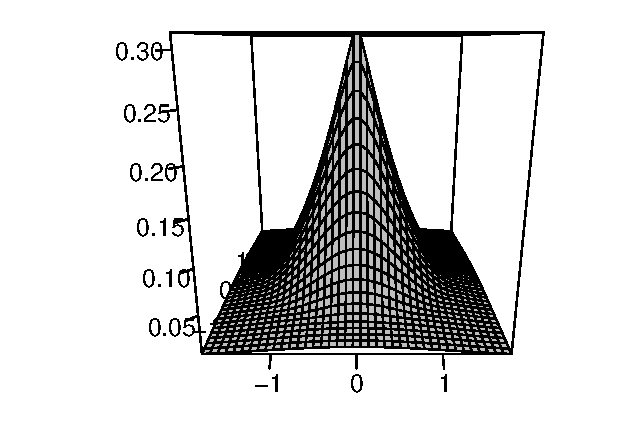
\includegraphics{./graphics/pollen.eps}
% \caption{Rape Seed Pollen Individual Dispersal Function.}
%     \label{fig:phi:klein}
% \end{center}
% \end{figure}

For this function,
the  threshold beyond which the
flow is calculated between centroids
only, is 100 m.


\medskip

\subsection{Individual dispersal function  of oilseed rape seeds}

The second function is the oilseed rape
seed individual dispersal function
proposed by Nathalie Colbach~\cite{Colbach2:2001}:
\begin{equation}
  \label{eq:dispersion:colbach}
  \phi\left(t\right)
  =
  \left\{
    \begin{array}{lll}
\dfrac{b \times c \times r^(c-2) \times \exp{ (-b \times r^c)}} {2.0*\pi}
    \end{array}
  \right.,\quad r=\left\|t\right\|.
\end{equation}
with $b = 1.38930$, $c= 2.08686$ and with
$t$ the  distance between the source  and the target points.
Distances are in meter.
See~Fig.~\ref{fig:phi:colbach}.

For this function,
the  threshold beyond which the
flow is supposed to be null is 21 m.

\begin{figure}[htbp]
  \begin{center}
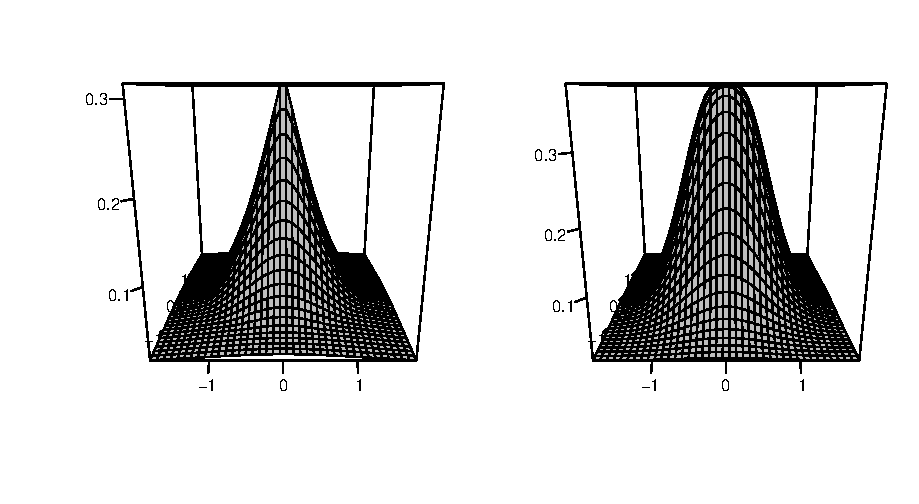
\includegraphics[width=15cm]{./VignetteDir/graphics/dispersion.eps}
%    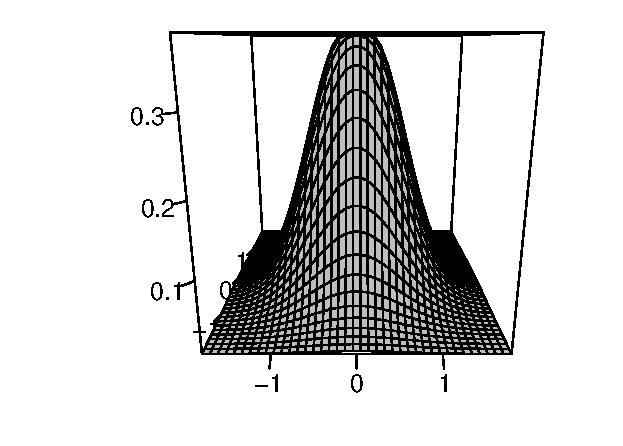
\includegraphics{./VignetteDir/graphics/seed.eps}
    \caption{Individual Dispersal Function of Pollen (on  the left) and
      Oilseed (on the right) Rape Seeds.}
     \label{fig:phi:klein}
    \label{fig:phi:colbach}
  \end{center}
\end{figure}

\subsection{How to modify or add individual dispersal functions}
\label{modifyfunctions}
The individual dispersal functions are coded in the C file
 \texttt{src/functions.cpp}.
To modify them, change the formulae expressions in the source code.
Don't forget they must be smooth functions.
Change also the DP* and DZ* constants
 in the file \texttt{src/caliconfig.h},
i.e the thresholds for  calculating dispersal between centroids only
and for considering that dispersal is zero, respectively.

In the delivered package, up to five dispersal functions 
can be defined. By default, the  DEFAULT\_NFUNCTIONS\footnote{
DEFAULT\_NFUNCTIONS is defined the file \texttt{src/caliconfig.h}.}
first functions are considered only.


After alteration of the source code, recompilation is required,
typically by using the standard R command: <tt>R CMD build RCALI</tt>
on top of your <tt>RCALI</tt> directory (see~\ref{howchanges}).







\part{A Small Glossary}
\label{glossary}
\begin{itemize}

\item\textbf{\hypertarget{cubmean}{$\widehat{\A}$ : integrated flow} in the cubature  method:}
\newline
For each
pair of convex subpolygons of a given pair
of polygons, the \hyperlink{mink}{Minkowski sum}
is calculated and triangulated.
$\widehat{\A}$ is the result of an adaptive cubature  integration
method
 on all the triangles.\\
Special cases:
when threshold distances have been set,
 $\widehat{\A}$ is automatically set to zero,
or calculated between centroids only,
beyond these distances (see~\ref{sec:steps}).


\item\textbf{\hypertarget{gridmean}{$\widehat{\A}$ : mean of the integrated flows} in the grid method:}
\newline
$\widehat{\A}$ is the sum over all the pairs of
convex subpolygons, 
of the mean of the calculated values over the replications, i.e:
$\widehat{\A} = \sum_{i=1}^{i=k}\sum_{j=1}^{j=r}\widehat{f}_{i,j}/r$,
where $k$ is the number of pairs of convex subpolygons and
$\widehat{f}_{i,j}$ is the calculated integrated flow 
between one such pair of subpolygons,
at the j$^{th}$ grid generation.\\
Special cases:
when threshold distances have been set,
$\widehat{\A}$ is automatically set to zero,
or calculated between centroids only,
beyond these distances (see~\ref{sec:steps}).



\item
\textbf{\hypertarget{gridcoefvar}{Coefficient of variation}  in the grid method:}
\newline
$CV = $\hyperlink{gridet}{$standard\ deviation$}/\hyperlink{gridmean}{$mean$}.

\item\textbf{\hypertarget{cubic}{Confidence Interval} in the cubature method:}
\newline
$IC = [\widehat{\A} - absolute\ error, \widehat{\A} + absolute\
error]$

\item\textbf{\hypertarget{mink}{ Minkowski sum of two polygons $A$ and $B$.}}
\newline
This sum is a polygon, denoted by $\check{A}\oplus B$.
It is the set of points $p$, such that:
$p= y-x, x \in A, y\in B$, i.e the set of points covered by $B$
when a vertex of $B$ is moved inside $A$.

\item\textbf{\hypertarget{reler}{Relative error} in the cubature method:}
\newline
$relative\ error = absolute\ error / result$




\item\textbf{\hypertarget{gridet}{Standard deviation}  in the grid method:}
\newline
$standard\ deviation =
\sqrt{\sum_{j=1}^{j=r}(\hat{f}_{.j}-\hat{f}_{..})^2 /(r-1)},$
where
$r$ is the number of replications, i.e
the number of grid generations,
$\hat{f}_{.j}$ the result of the grid integration at  replication $j$,
and $\hat{f}_{..}$ the  mean  result over the $j$ replications.

\end{itemize}


\part{Developer Guide}
\chapter{Implementation}

\section{Programme steps}

The main  steps have been described from the user's point of view
in Section~\ref{programme:does}.
Here, they are sketched
at the programming level. 



\subsection{Preprocessing}
Function \texttt{ReadPoly}:
\begin{enumerate}
\item
Read the polygons file and 
convert the coordinates into integers (-$>$\footnote{\label{ffr}Arrow is
  for a call to a subroutine.}\texttt {ReadCoord});
\item
Relocate the landscape (-$>$ \texttt {TranslatedParcel});
\item
For each polygon:
\enumerate
\item
remove aligned vertices and vertices forming a sharp spike;
\item
create convex subpolygons:
first, determine the essential diagonals, i.e
the diagonals which split the polygon into convex parts 
(-$>$ \texttt {Triangulate}),
 and then determine and store the convex subpolygons ((-$>$  \texttt  {HMAlgor}); 
\item
compute areas   (-$>$ \texttt {Area2}).
\end{enumerate}

\subsection{Calculation steps}

The function \texttt{suite} pilots the calculations process.
It realizes the following tasks:
\begin{enumerate}
\item
Create an object, \texttt {methode}, of class \texttt {methodGrid}
or \texttt {methodAdapt}.
\item
Call its method \texttt {VerifArgu} to verify its attributes.
\item
Pilot the loop on the required pairs of polygons:
for each of them, call the function \texttt {go}
which invokes
the methods \texttt {CalcR}
on  \texttt {methode} to perform the calculations,
\texttt {Print} to output the results on the screen,
and \texttt {PrintFic} to output them on a result-file.

\end{enumerate}

\subsection{Calculation by the grid method}

The method \texttt {CalcR}
of the class \texttt {methodGrid} is summarized by 
the following algorithm:

(The names of the devoted functions are between square brackets.)
 
\begin{algorithm}
  \caption{methodGrid::CalcR}
  \label{algo:grid}
\KwData{A pair of polygons $A$ and $B$, $nf$ individual  dispersal functions, user-defined parameters.}
\KwResult{Dispersal estimations from $A$ to $B$ by the
 grid method.}
Calculation of $mindist$, the minimal distance between the polygons.\\
\ForEach {dispersal function $\phi$ }{
\If{$mindist \geq$ threshold for function annulment}
{$result=0$}
\If{$mindist \geq$ threshold for calculation between centroids}
{$t$ = distance between centroids;  $result= \phi(t) \times area(A)
  \times area(B)$}
}
\tcp{In the other cases: one function at least should be integrated}

    \ForEach{pair of convex subpolygons $A_i$ and $B_j$ in $A$ and $B$}{
      Compute and store their Minkowski sum: $sommeM_{ij}$ [  \texttt{SommeMinkowski}];
      }
    \ForEach{ replication}{
      \ForEach{ pair of convex subpolygons $A_i$ and $B_j$}{
        Grid generation  [  \texttt{Integration}]:\\
        \ForEach{point $t$ of the grid}{
          \If{$t \in sommeM_{ij}$ [ \texttt{InPolyConvex}]}{
            $ar=area(A_i \cap (B_j - t))$;
            [  \texttt{ConvexIntersect}] \\
            \ForEach{ dispersal function $\phi$ to be integrated}{
              $result += \phi(t) \times ar$; 
              }
              }
              }
}
}
Compute the final results: means over the replications, standard deviation.
\end{algorithm}

\newpage
\subsection{Calculation by the cubature method}

The algorithm~\ref{algo:cub}
summarizes the tasks realized by
the method \texttt {CalcR} of
the \texttt{methodAdapt} class
(the names of the devoted functions are between square brackets).

$octo_{\phi}$ stands for the smallest octogon centered
  in (0,0) which includes the circle of radius equal
to the distance beyond which the dispersal function
$\phi$ becomes nul;
$octo_{\phi}$ is an
attribute of the \texttt{methodAdapt} class and
 is created by the class constructor.


\begin{algorithm}
  \caption{methodAdapt::CalcR}
  \label{algo:cub}
\KwData{A pair of polygons $A$ and $B$, $nf$ individual  dispersal functions, user-defined parameters.}
\KwResult{Dispersal estimations from $A$ to $B$ by the
cubature method.}
Calculation of $mindist$, the minimal distance between the polygons.\\
\ForEach {dispersal function $\phi$ }{
\If{$mindist \geq$ threshold for function annulment}
{$result=0$}
\If{$mindist \geq$ threshold for calculation between centroids}
{$t$ = distance between centroids;  $result = \phi(t) \times area(A)
  \times area(B)$}
\tcp{In the other cases: integration should be done}

  $stvertce=\emptyset; result=0$\;
    \ForEach {pair of convex subpolygons $A_i$ and $B_j$ of $A$ and
    $B$}{
      Compute and store the Minkowski sum: $sommeM_{ij}$; [ \texttt{SommeMinkowski}] \\
      \eIf{dispersal has no limit }{
        $S = sommeM_{ij}$\;
        }
{
\tcp{no dispersal beyond a given distance }
 $S = sommeM_{ij} \cap octo_{\phi}$
[ \texttt{TConvexIntersect}]\;
}
\If{$S \neq \emptyset$}{
\eIf{$(0,0) \in S$ \text{[ \texttt{InPolyConvex}]}}{
         $stvertce +=$  triangulation of $S$ from $(0,0)$ [ \texttt{Triangulate0}]\;}{
         $stvertce +=$  triangulation  of $S$ from any vertex
          [ \texttt{Triangulate}] \;}
} 
} \tcp{End of the loop over $A_i$, $B_j$}
Integration on the $stvertce$ triangles
for function $\phi$ [ \texttt{Adapt::Integration}];
} \tcp{End of the loop over the functions}
\end{algorithm}

\newpage
\section{Data structures}
\label{list:data}

The main data structures are described
in the following array:

\footnotesize
\begin{tabular}{|p{1.5cm}|p{3.5cm}|p{3.5cm}|p{5cm}|} \hline
{\bf Name} & {\bf Dimension} & {\bf Type} & {\bf Content} \\ \hline
Poly & npoly, nspoly, nvert, DIM &   tPolygoni (integer) & Polygons
coordinates, counterclockwise sorted, non-closed polygons  \\ \hline
ni & npoly, nspoly &   integer & ni$_{i,j}$: number of vertices 
in the subpolygon $j$ of the polygon $i$ \\ \hline
a & npoly &  integer & a$_i$: number of convex subpolygons
of the polygon $i$  \\ \hline
vertices & structure & tVertex (integer) & Linked list of the
ordered vertices of a polygon. Each element contains: \\ \cline{2-4}
 & V[DIM] & integer  & - coordinates of a vertex,  \\ \cline{2-4}
 & next & & - pointer to the next vertex
or to the head of the list if none, \\\cline{2-4}
& prev & & - pointer to the preceding vertex
or to the head of the list if none, \\\cline{2-4}
& vnum  & integer & - vertex indices   \\ \hline
sommeM & nvert, DIM & tPolygoni (integer) &   Minkowski Sum \\ \hline
intersection & id. as vertices & tdVertex (real) & Intersection of polygons \\ \hline
\end{tabular}
\newline
\noindent
npoly: number of polygons \\
nspoly: number of convex subpolygons in a polygon\\
nvert: number of vertices in a polygon\\
DIM: space dimension (here =2).

\normalsize

\newpage
\section{Functions list }
\label{liste:prog}
Some important functions are listed here.

(Words in {\em italic} refer to data structures.)

\footnotesize
\begin{tabular}{|p{2.5cm}|p{3.5cm}|p{7cm}|} \hline
 \hline
{\bf Function name} & {\bf File name} & {\bf
  Fonction} \\ \hline
ecrmess & util.cpp & Error message output and return to the calling
programme \\ \hline
libMem & util.cpp & Memory de-allocation \\ \hline
califlopp\_sd & fluxsd.cpp & Pilot \\ \hline
suite & go.cpp & Pilot the loop over the pairs of polygons \\ \hline
go & go.cpp & Pilot the treatment of one pair of polygons \\ \hline
\hline
read1Poly, read2Poly & read1Poly.cpp & Read the coordinates in format
1 and 2, resp. \\ \hline
ReadCoord  & readPoly.cpp & Read the polygons-file; verify the coordinates; scale
multiplication of the coordinates\\ \hline
ReadVertices & readPoly.cpp & Create {\em vertices}  \\ \hline
ReadPoly  & readPoly.cpp &  Create {\em Poly} with: \\
& & - aligned vertices removal  \\
& & - non-convex polygons splitting  \\ 
& & - areas computation \\ \hline
TranslateParcel & readPoly.cpp & Relocation of the polygons \\ \hline
\hline
ConvexIntersect & intersection.cpp & Convexity test and creation of
{\em intersection}  \\ \hline
Triangulate, HMAlgor, Area2 & geom.cpp &  Programmes of geometric
computation \\ \hline
SommeMinkowski & zoneintegration.cpp & Compute {\em sommeM}  \\
\hline
genrand\_real2 &mt19937ar.cpp & Random numbers generation$^1$ \\
 \hline
f0,f1,fX & functions.cpp & Individual dispersal functions \\ \hline
f\_ &  methodAdapt.cpp & The integrand for cubature method \\ \hline
Integration & methodGrid.cpp, &\\
& methodAdapt.cpp & Integration  \\ \hline
CalcR  & methodGrid.cpp, &\\
& methodAdapt.cpp & Compute one result   \\ \hline
Print, PrintFic & methodGrid.cpp, &\\
& methodAdapt.cpp & Output results on
screen and on file, resp.  \\ \hline
\hline
\end{tabular}
\normalsize
\paragraph{}
 See reference \cite{Matsumoto:1998}.

\paragraph{\textbf{Error codes:}}
The list and meaning of the errors codes can be found
in the file \texttt{calierror.h}.

\chapter{How to Modify }

It may be useful to know how to modify some parts.
Among them:

\begin{itemize}
\item
The individual dispersal functions:
see~Section~\ref{modifyfunctions}.
\item
The format of the polygons-file:
see the files \texttt{read1Poly.cpp}
and \texttt{read2Poly.cpp}.

\item
In interactive mode, the dialogue with the user:
see the file \texttt{fluxad.cpp},
and the \texttt{ReadArgu} method in the files
\texttt{methodGrid.cpp} and \texttt{methodAdapt.cpp}.


\item
Screen output:
see the file \texttt{go.cpp},
and the \texttt{Print} method in the files
\texttt{methodGrid.cpp} and \texttt{methodAdapt.cpp}.


\item
File output:
output on the result-file depend on the constant
OUTPUT\_FORMAT set in the file \texttt{caliconfig.h}.
They are carried on by
the \texttt{suite} function
and by the \texttt{PrintFic} methods in the files
\texttt{methodGrid.cpp} and \texttt{methodAdapt.cpp}.

\item
Erroneous polygons treatment:
the identifiers of the erroneous polygons
are made negative by the \texttt{ReadPoly}
function.
Their treatment depends on the constant
ERR\_POLY set in the file \texttt{caliconfig.h}.

\item
Memory allocation:
memory allocation is made via the macros CREER and NEW and
de-allocation  via the macros DETRU and FREE; they are coded in the
file
\texttt{calimacros.h}.

\item
Random number generator:
see the variable COPTIONS2 in the file \texttt{obj/subdir.mk}
and the corresponding code in \texttt{methodGrid.cpp}.

\item
Computing time measurement:
 see the file \texttt{timing.cpp}.
\item
Estimation of several integrals by the cubature method:
this possibility can be added
when  several integrals  have enough  similarity.
Estimation of all of them
can be made in one call. It is less time consuming.
For that, modify:
\begin{itemize}
\item
the function \texttt{f\_}  in the file \texttt{methodAdapt.cpp}:
the vector  \texttt{funvls}  should contain as many results
as integrals on output.
\item
the function \texttt{CalcR} in the file \texttt{methodAdapt.cpp}:
the first argument of the \texttt{Adapt} constructor should be
 equal to
the number of integrals. 
\item
the output operator in the file
\texttt{adapt/Adapt.h}:
it
should print as many results and absolute errors as integrals.
\end{itemize}
\end{itemize}

After alteration of the source code, recompilation is required:
see~paragaph~\ref{howchanges}.

% %%% 
% %%% 
% %%% %%% Local Variables: 
% %%% %%% mode: latex
% %%% %%% TeX-master: t
% %%% %%% End: 



%\part{Appendix}
%\appendix{}
%\include{annexe/annexe}
% Le copyright est dans le fichier COPYING: \include{copyright/copyright}

\part{Bibliography}
\bibliographystyle{alpha}

\bibliography{VignetteDir/biblio/biblio,VignetteDir/biblio/kien,VignetteDir/biblio/hm}

\textbf{
The red figures at the end of each reference refers to the pages
in the document.}



\end{document}

%%% Local Variables: 
%%% mode: latex
%%% TeX-master: t
%%% End: 

